\documentclass[letterpaper, 10 pt, conference]{ieeeconf}  % Comment this line out if you need a4paper

%\documentclass[a4paper, 10pt, conference]{ieeeconf}      % Use this line for a4 paper

\IEEEoverridecommandlockouts                              % This command is only needed if 
                                                          % you want to use the \thanks command

\overrideIEEEmargins                                      % Needed to meet printer requirements.

% The following packages can be found on http:\\www.ctan.org
\usepackage{graphics} % for pdf, bitmapped graphics files
%\usepackage{graphicx}
\usepackage[dvipdfmx]{graphicx}
\usepackage[dvipdfmx]{color}
\usepackage{epsfig} % for postscript graphics files
\usepackage{mathptmx} % assumes new font selection scheme installed
\usepackage{times} % assumes new font selection scheme installed
\usepackage{amsmath} % assumes amsmath package installed
\usepackage{amssymb}  % assumes amsmath package installed
\usepackage{multicol}
\usepackage{multirow}
\usepackage{url}
\usepackage{caption}
\usepackage[ruled,vlined]{algorithm2e}
%\include{pythonlisting}
\usepackage{algpseudocode}
\usepackage[dvipsnames]{xcolor}
\usepackage{cite}

\setlength\textfloatsep{5pt}

\title{\LARGE \bf
VCO-based Comparator: A Fully Adaptive Noise Scaling Comparator for High-Precision and Low-Power SAR ADCs
}

\author{Kentaro Yoshioka% <-this % stops a space
%\thanks{*This work was not supported by any organization}% <-this % stops a space
\thanks{
        {\tt\small yoshioka@elec.keio.ac.jp}}
}

\begin{document}

\maketitle
\thispagestyle{empty}
\pagestyle{empty}

%%%%%%%%%%%%%%%%%%%%%%%%%%%%%%%%%%%%%%%%%%%%%%%%%%%%%%%%%%%%%%%%%%%%%%%%%%%%%%%%
\begin{abstract}
VCO比較機ではdeadzone特性を使用することで自動的にIRN性能を入力に適した値に設定する。
The proposed adaptive time-domain (ATD) comparator automatically adjusts its input-referred noise performance according to the intermediate residual input level (?Vin) during conversion. Considering

入力に応じたオンデマンドのノイズと消費電力の比較器を提供。


\end{abstract}

%%%%%%%%%%%%%%%%%%%%%%%%%%%%%%%%%%%%%%%%%%%%%%%%%%%%%%%%%%%%%%%%%%%%%%%%%%%%%%%%
\section{Introduction}
As the number of sensors around us continues to increase with the advancement of IoT technology, high-precision, and low-power ADC circuits are necessary to percept precise environmental information with power-constrained sensors (e.g. battery, environmental power harvesting). In the past decade, there has been significant progress upon reducing the power of successive-approximation-register ADCs (SAR ADCs), which are suitable for CMOS scaling and do not require power-hungry opamps \cite{van201010,shikata20120,yoshioka201010,yoshioka20148,zhu201010,tai201411}. On the other hand, most of these low-power SAR ADCs have a limited dynamic range (SNDR$<$60dB); a SAR ADC with a wider dynamic range is demanded to adapt to a wider range of sensors and also reduce the burden of the ADC drivers. However, realizing a high-resolution and low-power capacitor digital-to-analog converter (C-DAC) and comparator is very challenging.

%IoT技術の進展により我々の身の回りのセンサ数は増え続けており、環境情報を精微にバッテリーレスでセンシングするには高精度かつ低電力なADC回路が必要である。この10年でref.\cite{van201010}を皮切りにCMOSスケーリングに好適であるsuccessive-approximation-register ADC (SAR ADC)の低電力化が大きく進み、多くの技術が提案された\cite{shikata20120,yoshioka201010,yoshioka20148,zhu201010,tai201411}。一方でこれらの低電力SAR ADCの多くはSNDR<60dBでありダイナミックレンジは限られており、よりダイナミックレンジが広いADCがあれば広範囲なセンサへの適応や前段アンプの負担を軽減することができる。しかしながらSAR ADCの高精度化はrealizing high-resolution capacitor digital-to-analog converter (C-DAC) and comparator with small power dissipation is very challenging. 

Conventionally, C-DACs were designed to satisfy the mismatch requirement and were designed with unit capacitors much larger than the kT/C noise requirement. Such use of large capacitors not only increases the power of the C-DAC itself, but also increases the  ADC driver and reference generation power as well, resulting in a large overhead. However, recent researches showed that capacitor matching requirements can be significantly relaxed by fully-digital background calibrations \cite{liu201012b,liu201112,mcneill2011all,mcneill2005split} and unit capacitors can be shrunk until kT/C limitations which greatly reduces the C-DAC power consumption. 
On the other hand, lowering the comparator noise is more challenging. Since the comparator is the only pure analog component in SAR ADCs, designers must face tradeoffs of noise, power consumption, speed, and PVT variation tolerance.

We propose a VCO-based comparator that can fully adapt its noise performance depending on the input voltage difference ($\Delta V_{in}$), to minimize the power consumption of a high-precision comparator\cite{yoshioka201413b}. The input voltage difference is integrated as a time difference via the VCO, where the integration continues as long as the time difference is below a certain threshold, defined by the phase detector deadzone. Since this integration opens an "eye" (as in high-speed IO circuits) as the VCO oscillation continues, we name this \textit{eye-opening} technique. For large $\delta V_{in}$, the oscillation is terminated within a single cycle, and on the other hand, with small $\Delta V_{in}$, the oscillation continues until the integrated time difference exceeds the threshold. Such operation not only adapts the comparator noise performance but since the comparator power is proportional to the number of oscillations, the power also scales with $\delta V_{in}$ and minimizes the comparator power.
Compared to the data-driven-noise-reduction (DDNR) comparator\cite{harpe201310b}, which switches between two noise modes based on the comparator's metastable state, the comparator power can ideally be reduced by half.

We demonstrate the concept of the VCO-based comparator with a 13 bit SAR ADC fabricated in 65nm CMOS. The ADC achieves peak SNDR of 66 dB at 1 MS/s with a FoM of 29 fJ/conv.-step. Since the VCO-based comparator is mainly based on inverters and other simple logic cells, benefits can be granted by process scaling.
To the best of the author's knowledge, the VCO-based comparator is the first comparator to achieve a fully adaptive noise performance reflecting the input differential levels, and comparators based on eye-opening techniques have been used in a variety of low-power, high-resolution (12-15 bit) SAR ADCs \cite{ding20190, luo2020input, hsieh20180, li2019design, li202065, almarashli2017nyquist, shim2017edge, zhu201914, pan202012, lee2019fast, vogelmann2020efficient}.

This paper expands on ref.\cite{yoshioka201413b} with detailed analysis of the VCO-based comparator, including its operating principle, noise characteristics, detailed circuit implementation, and noise tolerance under PVT variations.
The paper is organized as follows: Chapter 2 describes the challenges of conventional high-precision comparators, Chapter 3 describes the principle and analysis of the VCO-based comparator, Chapter 4 describes the circuit implementation, and finally Chapter 5 presents the measurement results and concludes with a summary.

%本論文ではref.\cite{yoshioka201413b}から発展させVCO比較器の動作原理やノイズ特性、詳細回路インプリ、そしてPVTばらつき下におけるノイズ変動耐性といった詳細な解析結果を追加する。本論文の構成は以下である。二章では従来高精度比較器の課題、3章ではVCO比較器の原理と解析、4章では回路インプリについてそして最後に5章で測定結果を示し最後にまとめる。


%\section{Comparison of systematic comparator power consumption}
\section{Conventional low-power low-noise comparators}
\begin{figure}[ht!]
\centering
 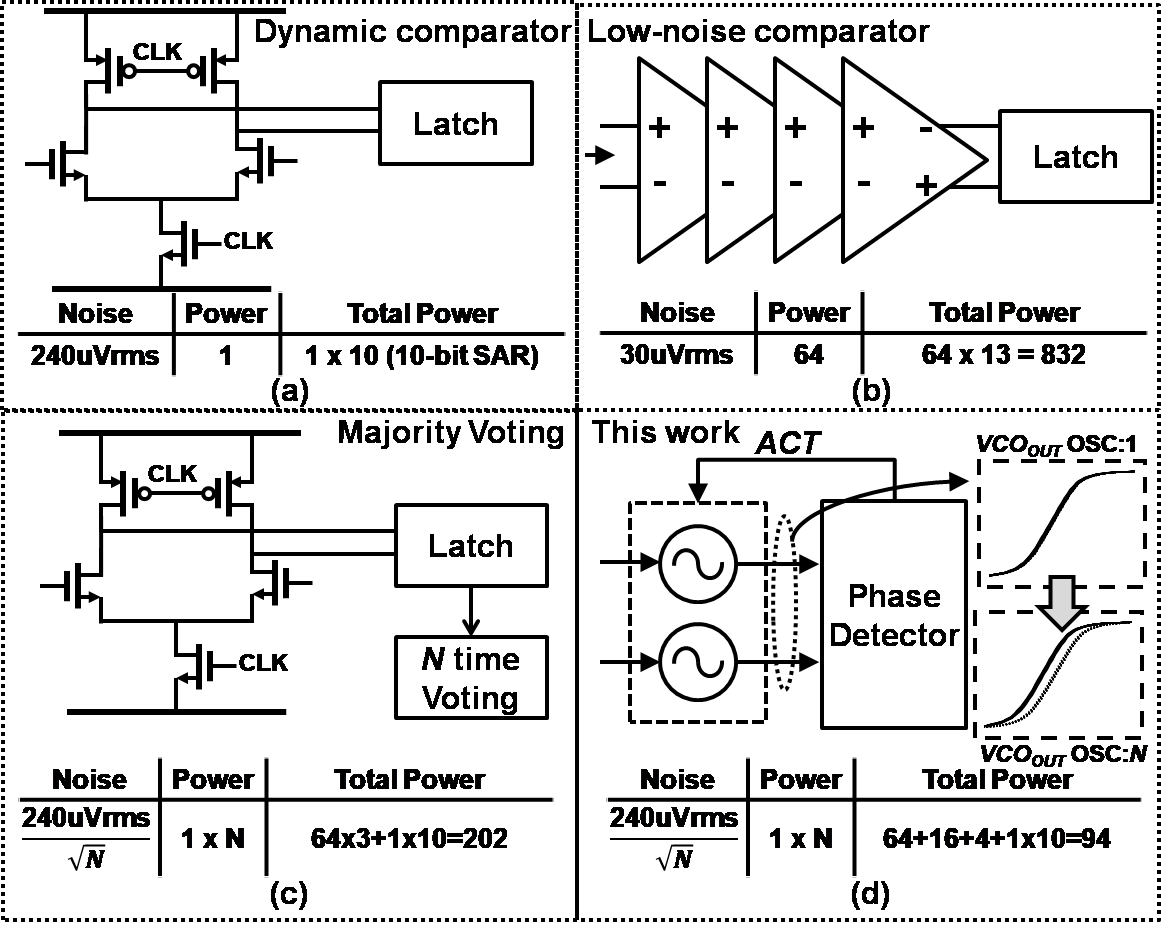
\includegraphics[width=0.5\textwidth]{figs/fig1.png}
  \captionsetup{font=footnotesize}
  \caption{\textbf{ADC}}
  \label{fig1}
\end{figure}
\begin{figure}[ht!]
\centering
 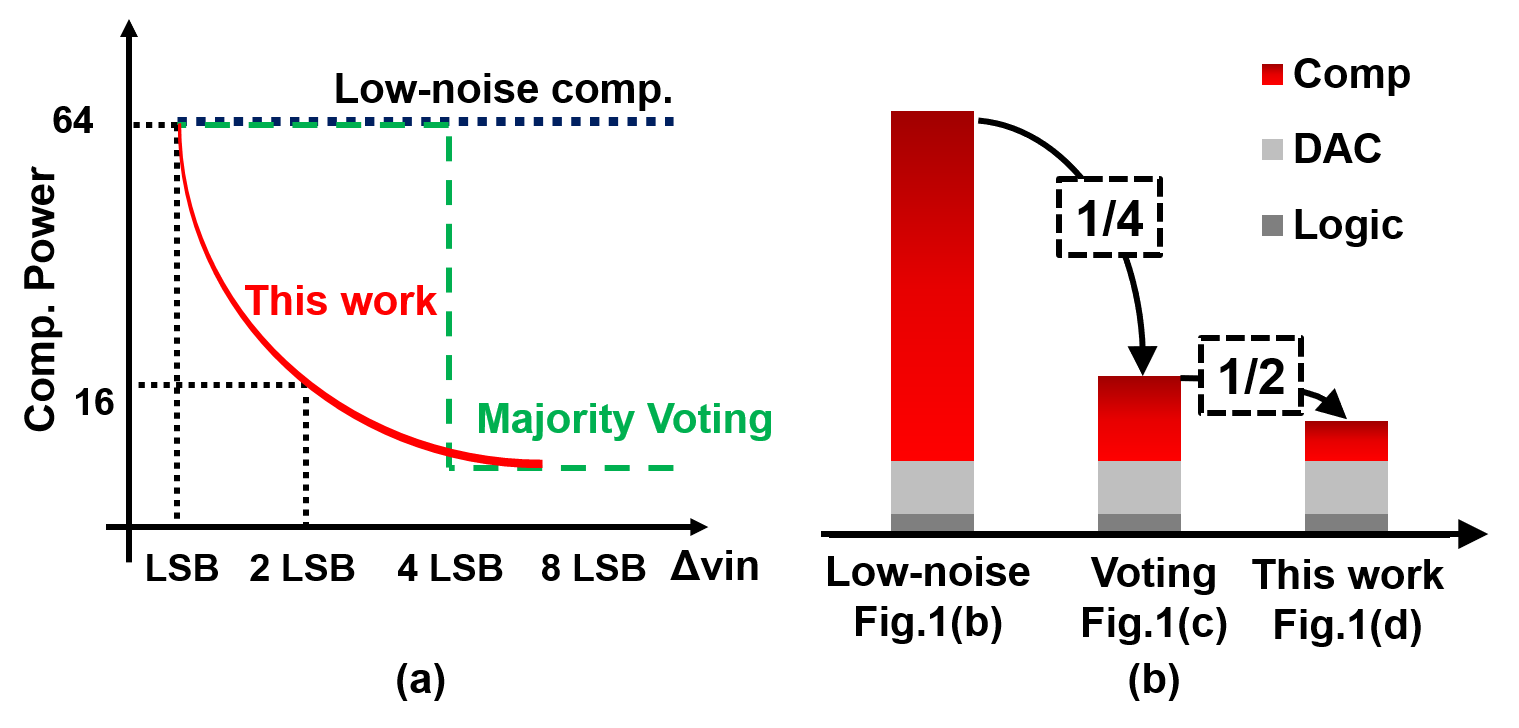
\includegraphics[width=0.5\textwidth]{figs/fig2.png}
  \captionsetup{font=footnotesize}
  \caption{\textbf{ADC}}
  \label{fig2}
\end{figure}
\begin{figure}[ht!]
\centering
 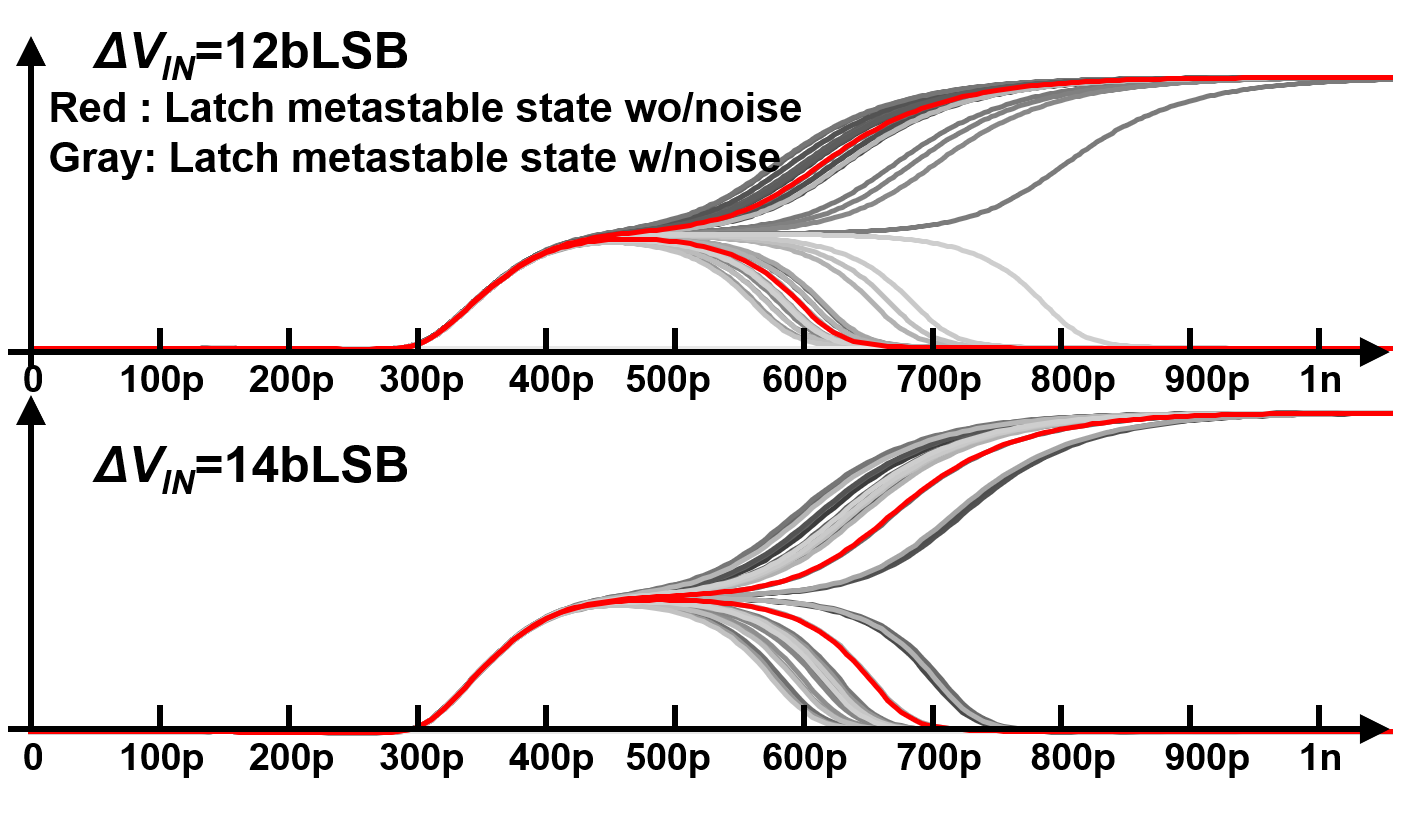
\includegraphics[width=0.5\textwidth]{figs/conventional-strongarm.png}
  \captionsetup{font=footnotesize}
  \caption{\textbf{ADC}}
  \label{meta}
\end{figure}

Fig.\ref{fig1}(a) shows a typical comparator used in low-power SAR ADCs\cite{miyahara2008low}. Although the noise can be reduced by limiting the bandwidth of the preamp stage, a typical design has an input-referred noise (IRN) around 10-bit resolution. Fig.\ref{fig1}(b) shows a comparator used in 14-bit SAR ADC \cite{hesener200714b}: the comparator IRN is reduced by cascading preamp stages before the latch. However, during the successive approximation (SA) conversion, comparator input differential voltage ($\Delta V_{in}$) differs each cycle (Fig.\ref{fig2}(a)) Moreover, during the SA conversion, $\Delta V_{in}<$LSB only occurs once, which is the situation when comparator noise requirement is most strict. The comparator noise requirement is relaxed at other cycles and utilizing a low-noise comparator for all of the cycles is inefficient. 

To cut down the comparator power, ref.\cite{harpe201310b} propose a data-driven noise reduction (DDNR) technique, where the comparator triggers majority voting when the $\Delta V_{in}$ is sufficiently small for comparator meta-stability \cite{shikata20120}. The comparator output is decided given the result of $N$ time majority voting, and comparator IRN improves as:
\begin{eqnarray}
    \centering
    V_{voting} = \frac{V_{noise}}{\sqrt{N}}
    \label{voting}
\end{eqnarray}
By switching to a low-noise comparator using voting only when $\Delta V_{in}$ is small, the systematical comparator power can be greatly reduced.
Here, we conduct a simple analysis of the systematic comparator power of the conventional techniques. Ideally, to halve the comparator IRN, 4x much power must be consumed. Therefore, when the power of the 10-bit resolution comparator is normalized as 1, the power of the 13-bit comparator can be described as:
\begin{eqnarray}
    \centering
    P_{13bcomp} = 1 \times 4^{13-10} = 64
    \label{13b}
\end{eqnarray}
Then, the total comparator power of 13-bit SAR ADC will be:
\begin{eqnarray}
    \centering
    P_{total(Fig.1(b)} = 64 \times 13 = 832
    \label{sar13b}
\end{eqnarray}
Next, we will assume an ideal DDNR done by 10-bit comparator, where majority voting is triggered when $\Delta V_{in}$ is smaller than 4LSB (corresponding to 11-bit resolution).
\begin{eqnarray}
    \centering
    P_{total(Fig.1(c)} = 64 \times 3 + 1 \times 10 = 202
    \label{ddnr}
\end{eqnarray}
The analysis shows that comparator power can reduced by over 1/4 with DDNR. $\Delta V_{in}$ versus comparator power is shown in Fig.\ref{fig2}(b), where the power of the majority voting is plotted in the dashed green line. 
DDNR can significantly reduce the comparison power by switching the noise performance of the comparator according to the input.
On the other hand, the DDNR comparator can only switch between two noise performances, and as a result, the power consumption jumps up when $\Delta V_{in}$ exceeds 4 LSB. 
However, for $\Delta V_{in}$ = 4 LSB, the required comparator noise performance is also equivalent to 4 LSB; it is inefficient to use a comparator with noise performance of 1 LSB.
Thus, the comparison energy can be further reduced by finely switching the comparator noise performance  reflecting $\Delta V_{in}$ "on-demand". 

If the metastable time of the comparator is inversely proportional to $\Delta V_{in}$, on-demand noise control can be achieved by switching the DDNR voting count according to the metastable time.
However, the metastable time of the voltage domain comparator does not have a direct correlation with $\Delta V_{in}$, making such an implementation difficult. For reference, Fig.\ref{meta} shows the metastable state of the latch response when $\Delta V_{in}$ of 2 LSB and 0.5 LSB are given to the 2-stage comparator \cite{miyahara2008low} with 10-bit noise. Without any noise, the regeneration time is inversely proportional to $\Delta V_{in}$ as shown in the red. On the other hand, when noise is present, the latch often opens early due to noise effects and $\Delta V_{in}$ cannot be estimated directly from the regeneration time.

We propose a VCO-based comparator that can fully adapt its noise performance reflecting the $\Delta V_{in}$ condition. Thus, the ideal VCO-based comparator's power will fully depend on $\Delta V_{in}$, as shown in Fig.\ref{fig2}(b). The systematic VCO-based comparator power consumption in this case can be calculated as:
\begin{eqnarray}
    \centering
    P_{total(Fig.1(d))} = 64+16+4+1\times 10=94
    \label{ddnr}
\end{eqnarray}
which is half of that of the DDNR with majority voting (Fig.\ref{fig2}(c)). 
The specific operating principle of the VCO-based comparator is described in the next chapter.

%またTime domain comparators such as delay comparator \cite{agnes20089} はプロセススケーラビリティと低電力動作能力を持ち、発展が期待されている. 一方でこれらのnoise characteristics are not enough for high-resolution ADCs.

\begin{figure*}[ht!]
\centering
 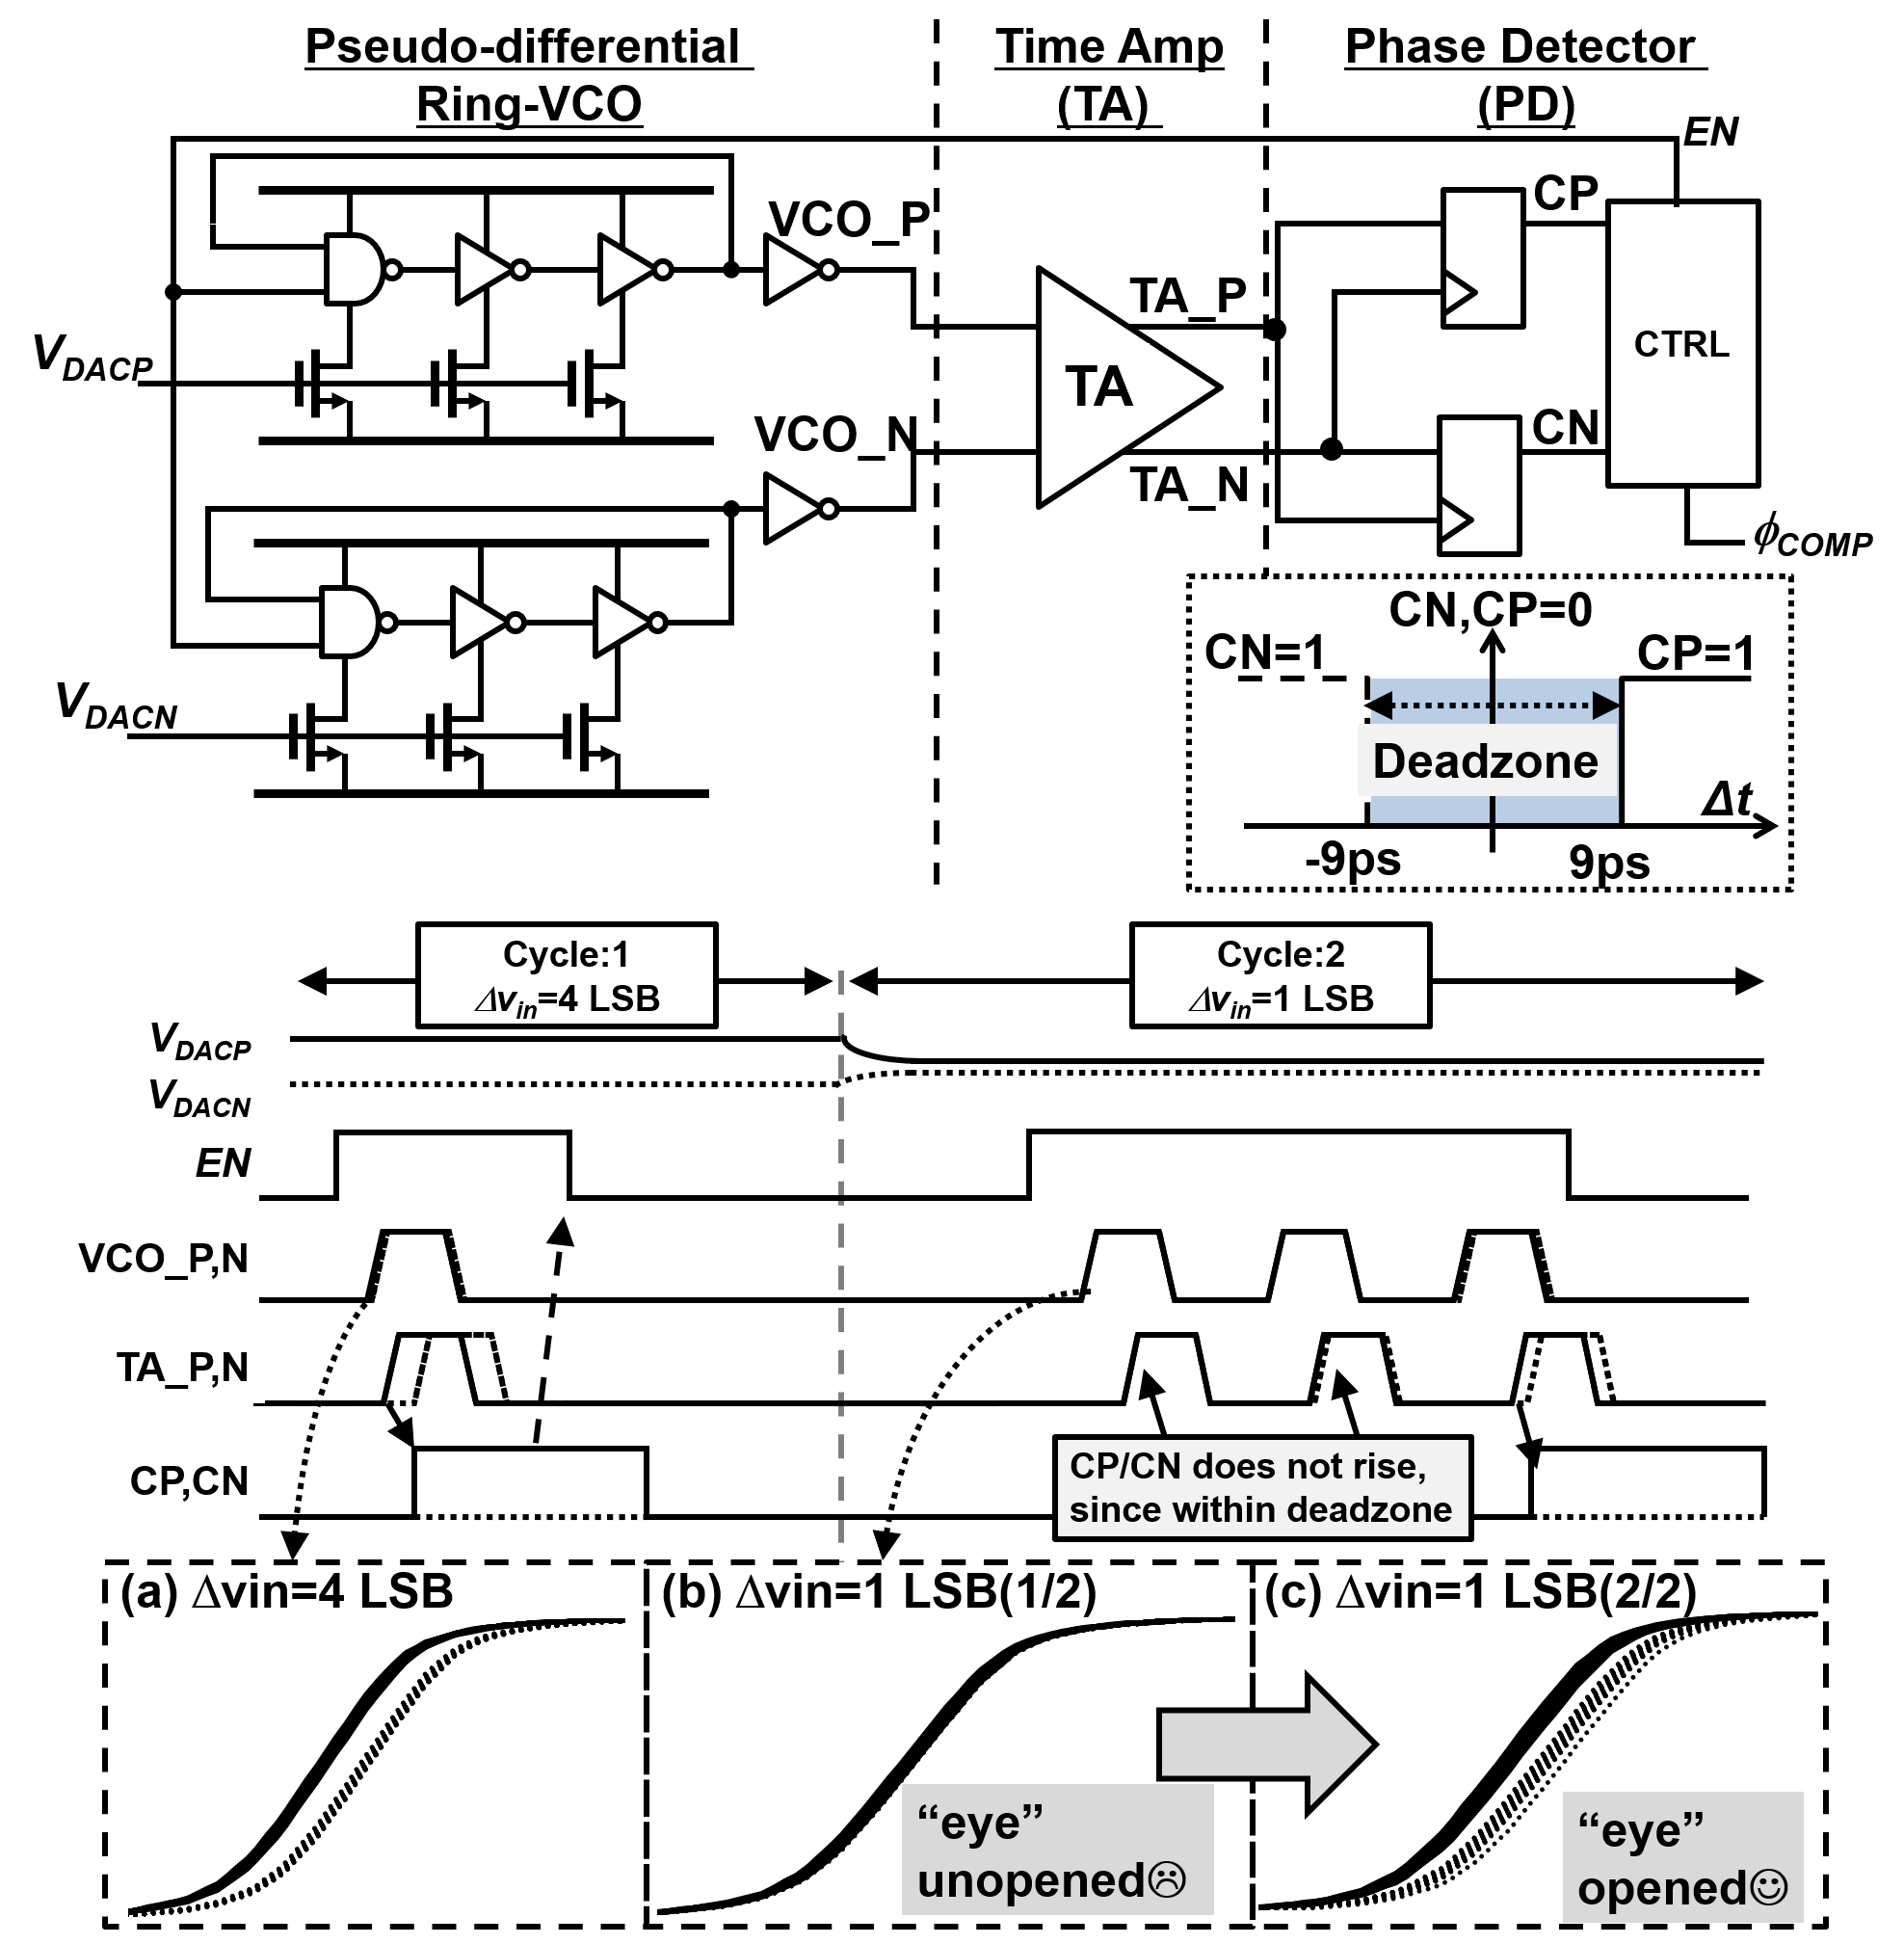
\includegraphics[width=0.9\textwidth]{figs/full.png}
  \captionsetup{font=footnotesize}
  \caption{\textbf{ADC}}
  \label{schema}
\end{figure*}

\section{VCO-based comparator}
\subsection{VCO-based comparator Fundamentals}
Fig.\ref{schema} shows the conceptional schematic of the VCO-based comparator. Similar to delay line based comparators\cite{agnes20089}, the C-DAC analog voltages($V_{DACP}$, $V_{DACN}$) are given to control the oscillating frequency of the ring oscillator. We utilize a time amplifier (TA)\cite{lee20089} to amplify the time difference between the VCO outputs ($VCO_P$, $VCO_N$). Finally, the TA outputs ($TA_P$, $TA_N$) are connected to the phase detector, which resolves the comparison results.

The lower part of Fig.\ref{schema} shows the VCO-based comparator operation in the case of large and small $\Delta V_{in}$, respectively. In this example, at cycle 1, $\Delta V_{in}$ is fairly large ($>$4 LSB) where the VCO-based comparator adaptively operates as a delay line comparator. When $EN$ rises, the VCOs are "enabled" and pulses start to travel through the ring-VCO inverter cells. The pulses reach the TA and their time difference is amplified. In this case, $TA_P$ rises faster than $TA_N$ with sufficient margins and the D-FF-based phase detector resolves the comparison results: CP=1 and CN=0. Once the comparison results are obtained, $EN$ is set down to “disable” the ring-VCO, which resets the ring-VCO phase state and prevents unnecessary oscillations.

Next, the comparator operation with small $\Delta V_{in}$ (Cycle 2 in Fig.\ref{schema}) is explained. Similarly, $EN$ rise and the pulses transmit through the VCOs. Fig.\ref{schema}(a) and (b) plot the VCO outputs of 50-times noise simulation with $\Delta V_{in}$ of 4 and 1 LSB, respectively. Note that in (b), an “eye” is not opened because the VCO jitter is larger than the input-dependent time difference. In such conditions, the comparator cannot make correct decisions and noise reduction is required.

In VCO-based comparators, the event of small $\Delta V_{in}$ is detected by exploiting the deadzone property of the D-FF based PD. It is known that D-FF based phase detectors (PDs) require a finite setup and hold time to produce an output: if the input time difference between the data and the clock is too short ($<$9ps in 65nm CMOS), a "deadzone" occur where the output does not respond.
As in cycle 2 of Fig.\ref{schema}, when the $TA_P$ and $TA_N$ difference is small and within the deadzone, the VCO automatically continues the oscillation (or signal integration) until the time difference is large enough to exceed the deadzone. Such utilization of VCOs and the deadzone allows us to configure the comparator noise adaptively reflecting the $\delta V_{in}$ level.
In Fig.\ref{schema}, the TA output exceeds the deadzone after 3 oscillations. Fig.\ref{schema}(c) shows the noise simulation of VCO output after 3 oscillations and “eye-opening” is observed.

\begin{figure}[ht!]
\centering
 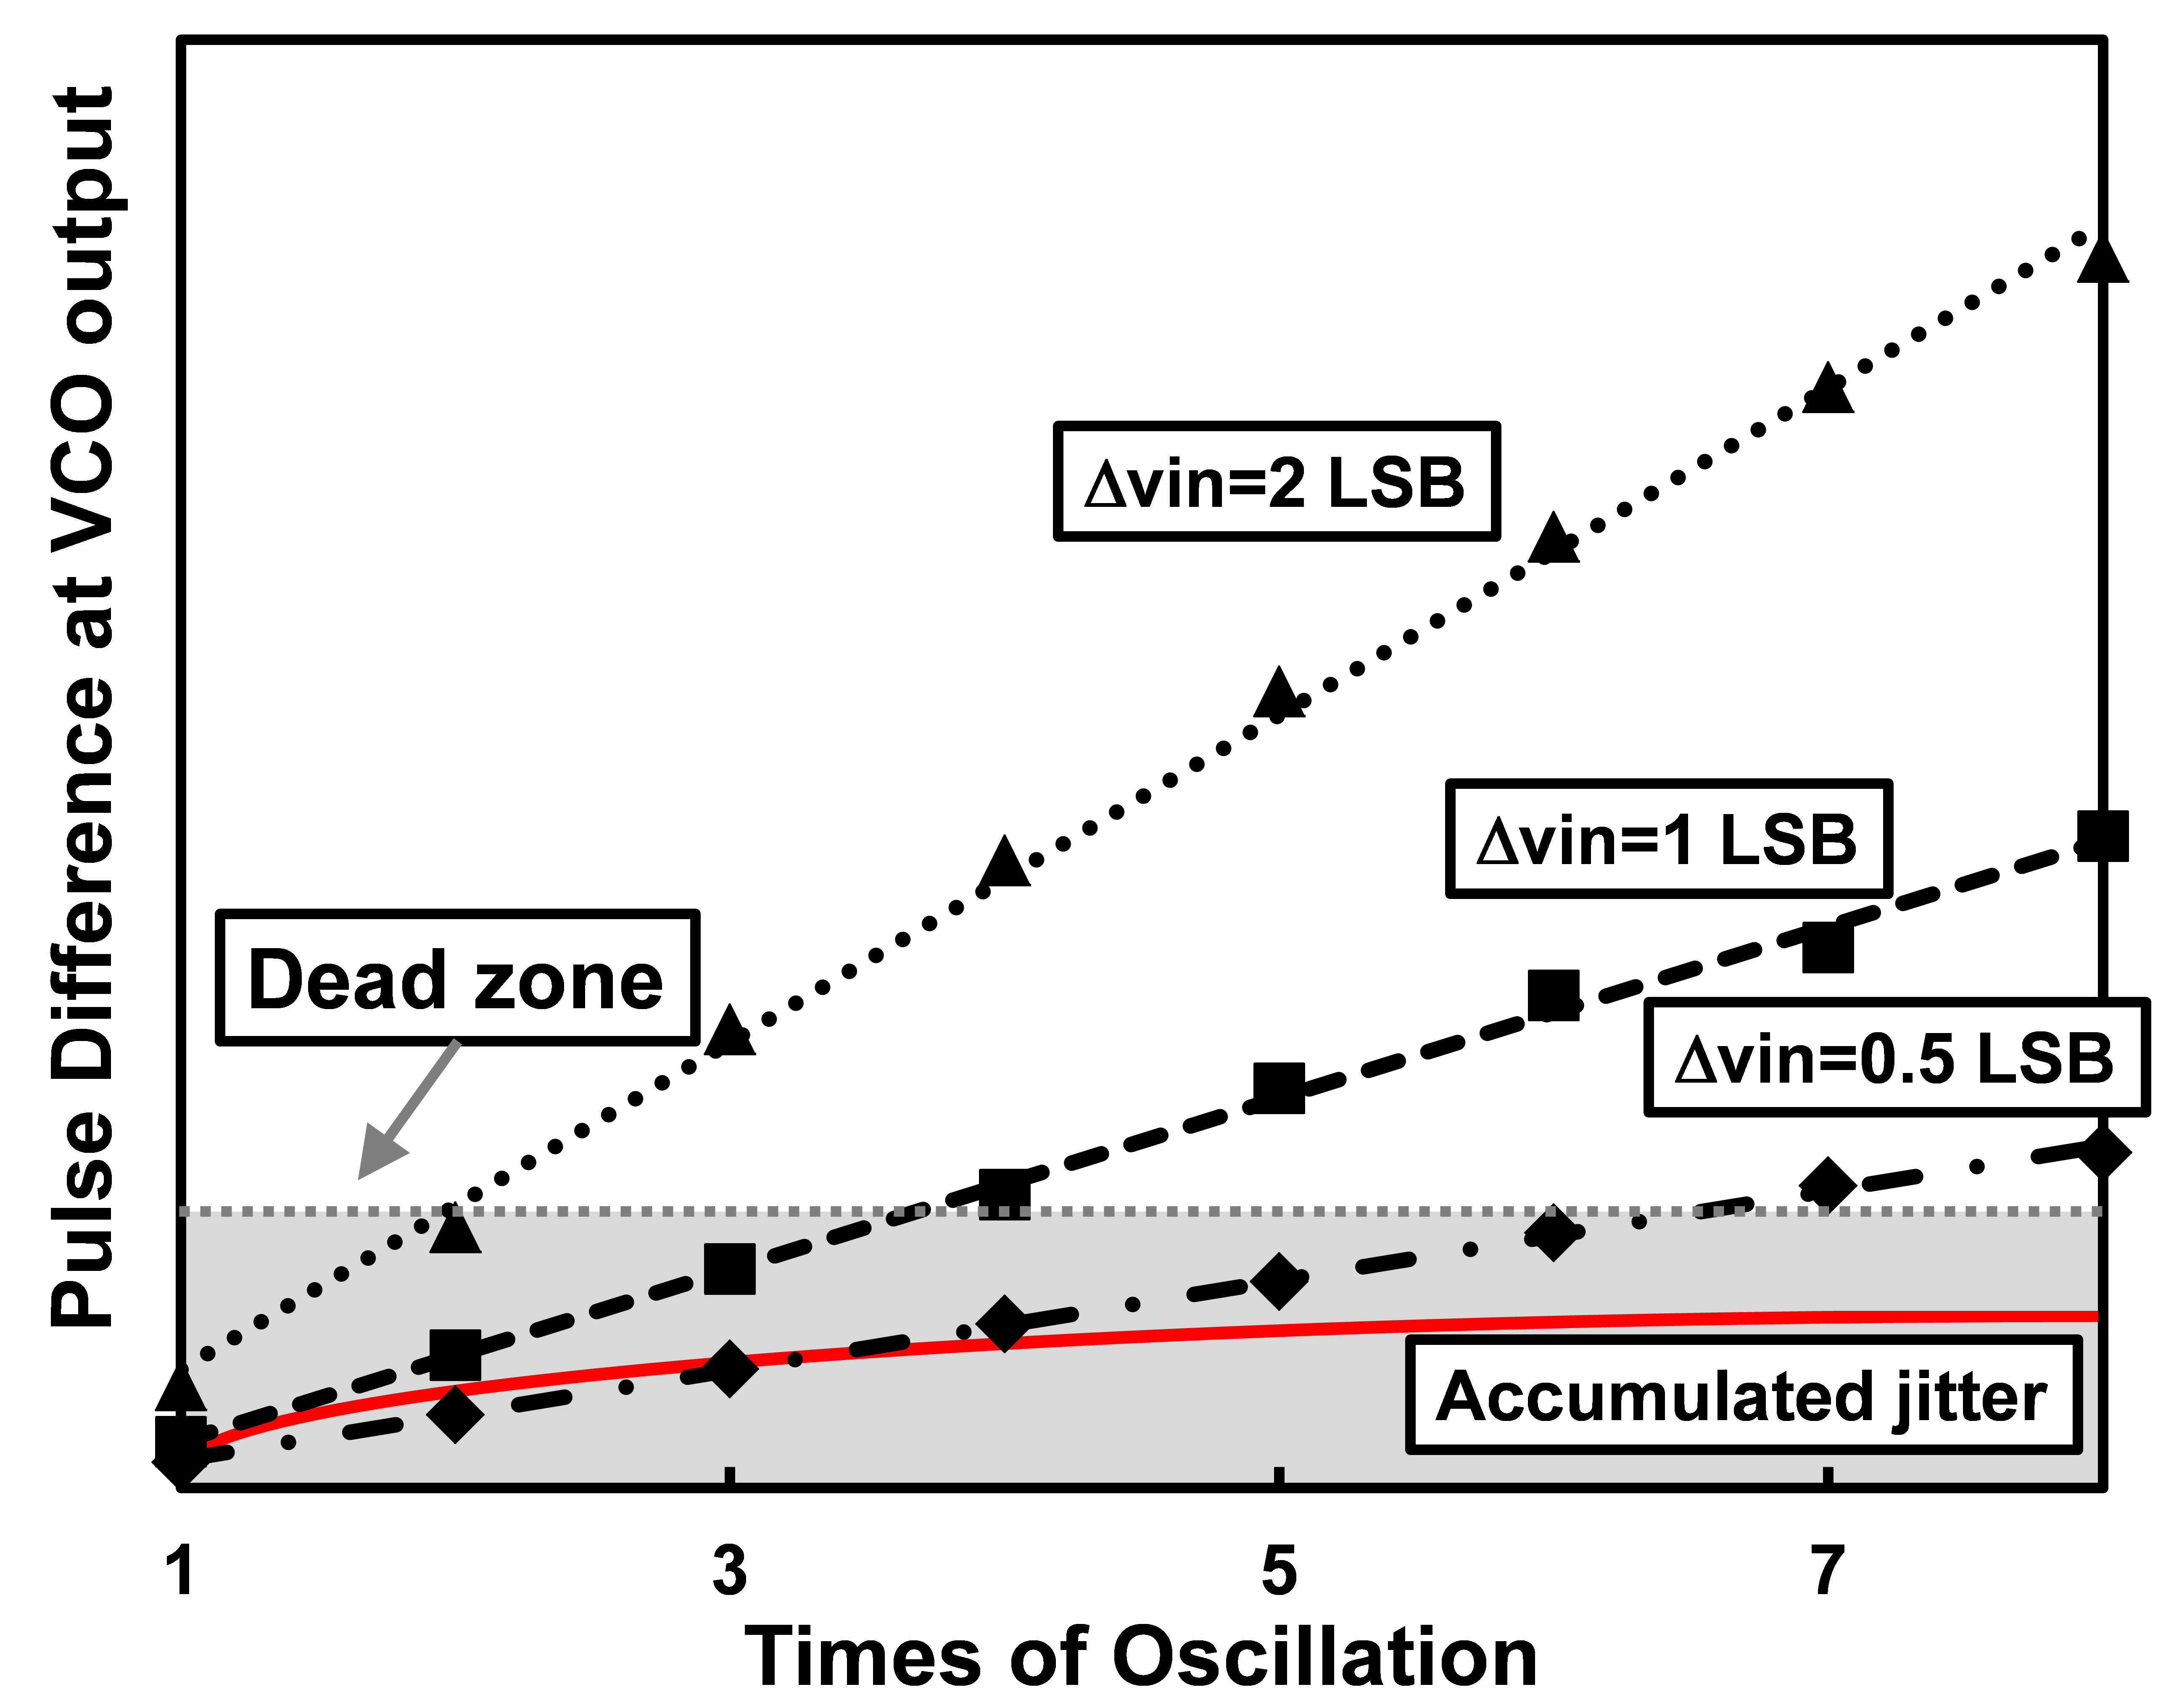
\includegraphics[width=0.5\textwidth]{figs/fig5.png}
  \captionsetup{font=footnotesize}
  \caption{\textbf{ADC}}
  \label{fig5}
\end{figure}

An initial study of the VCO-based comparator's noise reduction is explained with the aid of Fig.\ref{fig5}, where the simulation result of the Number of Oscillations ($N$) vs VCO pulse difference is plotted for $\Delta V_{in}$ of 11-bit, 12-bit, and 13-bit LSB, respectively. We can observe that $N$ and pulse difference have a linear relationship of $\alpha N$ and $\alpha$ is decided by the VCO voltage conversion gain. On the other hand, the accumulated jitter is proportional to $\sqrt N$\cite{hajimiri1999jitter,abidi2006phase}. In the case of $\Delta V_{in}$ = 13-bit LSB, even though the jitter may be dominant at 1-3 times of oscillation, the signal-dependent pulse difference will overcome the jitter as $N$ increase. The area in gray indicates the deadzone: as long as the pulse difference is within the deadzone, the oscillation will continue. The detailed VCO-based comparator's noise design guide is given in the next section.
%Therefore, by careful design of the deadzone and VCO jitter, we can design VCO-based comparators with the desired noise performance.

\subsection{Noise design guide of VCO-based comparators}
The most important aspect of designing a high-precision comparator is the noise design; this section discusses the noise design guidelines for VCO-based comparators. Although the noise analysis of VCO-based comparators is described in detail in ref.\cite{luo2020input, ding20190}, comparator design guidelines are not discussed. Designing a VCO-based comparator satisfying a desired noise involves two major steps.
\begin{itemize}
\item Firstly, the VCO block is designed as a delay line based comparator which satisfies a certain speed and noise. Since accurate comparison can be achieved by eye-opening operation, as a rule-of-a-thumb, the noise of the delay line based comparator should be around $4\times$ worse than the target IRN to obtain sufficient power savings.
\item To obtain the peak noise performance, the VCO-referred deadzone is tuned with the aid of TA gain.
\end{itemize}

The first step is to design the VCO block as a delay line based comparator satisfying a certain noise.
Following ref.\cite{timecomp}, the jitter of a unit delay stage can be calculated as:
\begin{eqnarray}
    \centering
    jitter_{unit} = \frac{\sqrt{C_L\beta k \rm{T}}}{I_{DS}}
    \label{jit}
\end{eqnarray}
where $\beta$ is the product of $g_m$, $r_o$, and noise factor $\gamma$ and $I_{DS}$ is the inverter current when $V_{in} = V_{DD}/2$ and k is Boltzmann’s constant.
The unit stage's voltage-time conversion gain can be obtained with the analysis in ref.\cite{timecomp} as: 
\begin{eqnarray}
    \centering
    \rm{Gain} = \frac{g_mC_LV_{DD}}{2I_{DS}^2}
    \label{gain}
\end{eqnarray}
From eq.(\ref{jit}) and (\ref{gain}), the IRN($IRN_{DL}$) of the $N_{inv}$ stage delay line based comparator with NMOS voltage-time conversion can be derived as:
\begin{eqnarray}
    \centering
    IRN_{DL} = \frac{\sqrt{jitter}}{\rm{Gain}} = \frac{1}{\sqrt{N_{inv}C_L}}\frac{2I_{DS}\sqrt{2\beta k\rm{T}}}{V_{DD}g_m}
    \label{delaylineIRN}
\end{eqnarray}

\begin{figure}[ht!]
\centering
 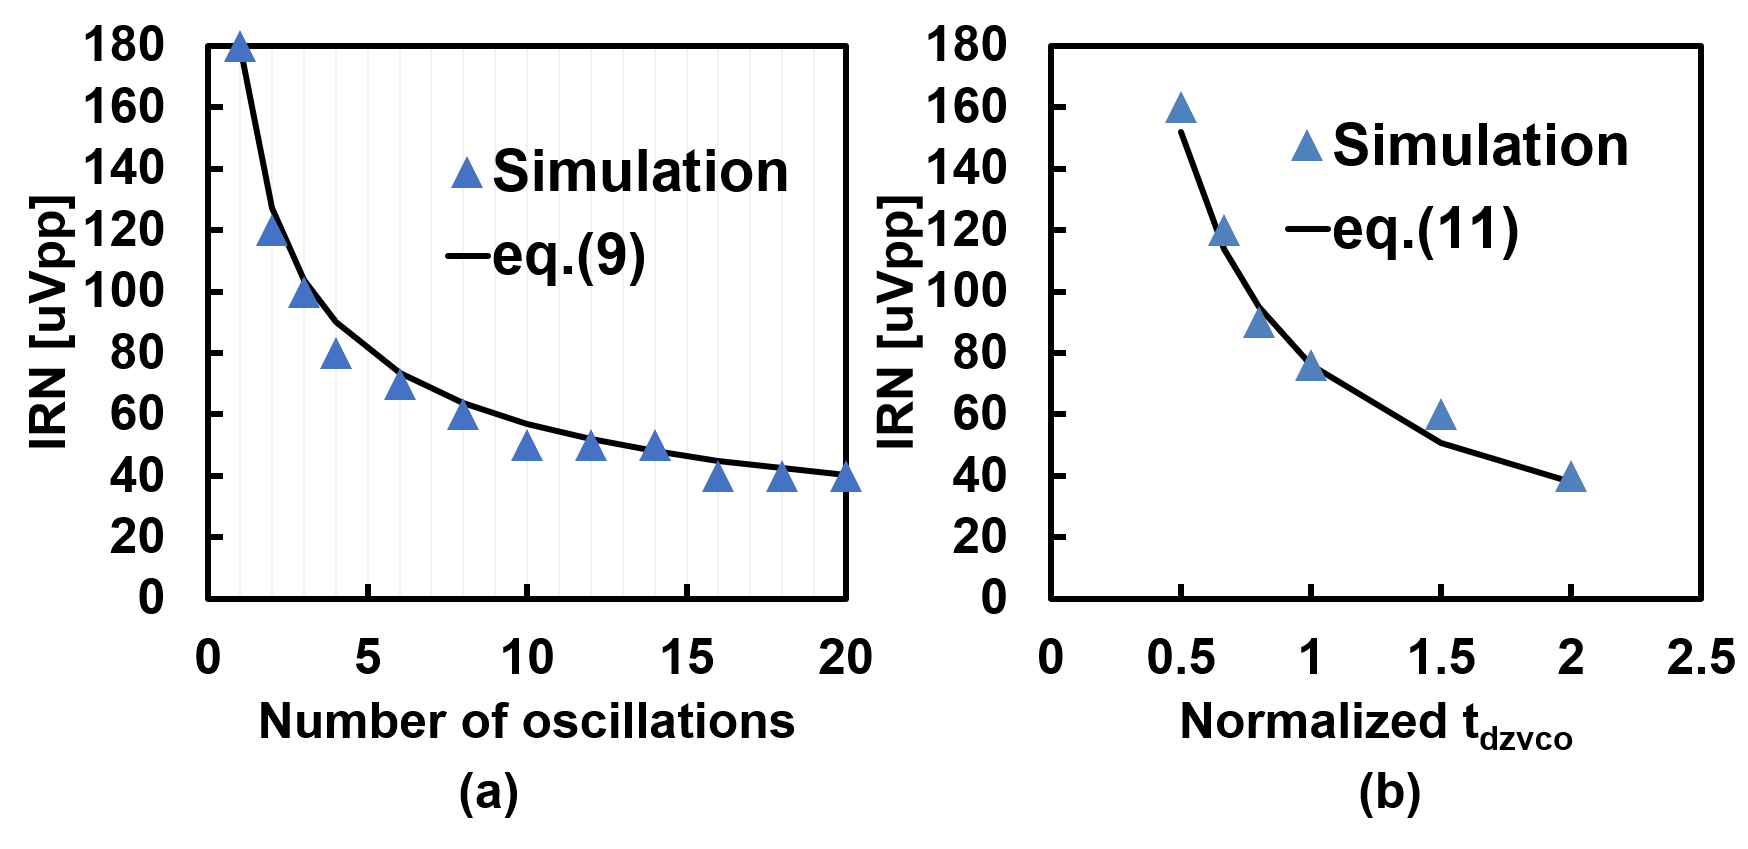
\includegraphics[width=0.5\textwidth]{figs/analysis.png}
  \captionsetup{font=footnotesize}
  \caption{Eq.(9)とノイズシミュレーションによって確認したVCO比較器ノイズの比較。ほぼeq.(9)に沿ったノイズ性能が得られることを確認できた。}
  \label{nocnoise}
\end{figure}

Then, as discussed in fig.\ref{fig5}, the signal is integrated by oscillating the VCO to improve the IRN.
The relationship between the number of oscillations $N$ and IRN is as follows.
\begin{eqnarray}
    \centering
    IRN_{VCO} = \frac{IRN_{DL}}{\sqrt{N}}
    \label{vcoIRN}
\end{eqnarray}
Fig.\ref{nocnoise} confirms that eq.(\ref{vcoIRN}) holds in transient noise simulation. The state at the oscillation frequency = 1 is equivalent to $IRN_{DL}$ as a delay line comparator, and the simulation confirms that the noise improves with the square root of the oscillation frequency.

%ちゃんとした解析を足す。。?
Due to the adaptive noise performance characteristics of the VCO comparator, the noise requirements of the $IRN_{DL}$ itself are relaxed. As a rule of thumb, to minimize the overall comparator power, the target $IRN_{DL}$ should be about four times worse than the peak IRN to achieve a good balance between the VCO comparator power consumption and noise. %For example, we can try to maximize the input transistor $g_m$ in eq.(\ref{delaylineIR}).

% deadzoneの効果。VCOからみたdeadzoneはDFF deadzone/TA gain。
Next, we will show the noise design of a VCO comparator by tuning the VCO-referred deadzone.
First of all, due to the time amplifier, the deadzone seen from the VCO output ($t_{dzvco}$) is compressed by the TA gain $G_{TA}$.
\begin{eqnarray}
    \centering
    t_{dzvco} = \frac{t_{dz}}{G_{TA}}
    \label{dzvco}
\end{eqnarray}
Importantly, the IRN of the VCO comparator is inversely proportional to the deadzone, as analyzed in ref.\cite{luo2020input, ding20190}. Thus, from eq.(\ref{dzvco}), we can derive:
\begin{eqnarray}
    \centering
    IRN \propto \frac{IRN_{DL}}{t_{dzvco}} = \frac{IRN_{DL}\times G_{TA}}{t_{dz}}
    \label{irn}
\end{eqnarray}
Interestingly, this shows that by tuning $G_{TA}$, we can directly tune the VCO comparator IRN. Note that directly tuning $T_{dz}$ is difficult, and tuning $IRN_DL$ has a large impact on the comparator power. On the other hand, $G_{TA}$ can be easily tuned by the capacitive load, as described in the next chapter, and provides great flexibility in the comparator noise design. To confirm Eq.(\ref{irn}), we used transient noise simulation and swept $t_{dzvco}$ by configuring the TA gain and measured the comparator IRN (Fig.\ref{nocnoise}(b)). It can be seen that the simulated IRN matches eq.(\ref{irn}) well. We would also like to note that the actual IRN also includes the noise from TA and PD. In our design, the total noise of TA and PD was about 1/4 of the entire IRN, so there is no significant deviation from eq.(\ref{irn}).

%\subsection{Power Saving Characteristics}
%提案したVCO比較器は入力レベルに応じたエネルギーを消費する。まず特性を確認するため、入力差を振ったシミュレーション結果のVdi%f vs Energyをプロット。
%VCO比較器はノイズをかんたんにプログラム可能。上記IRNは理論限界
%10, 10.5, 11, 11.5, 12, 12.5, 13, 13.5
%low noise vs ddnr vs vco comp.

\subsection{PVT drift resistance}
\begin{figure}[ht!]
\centering
 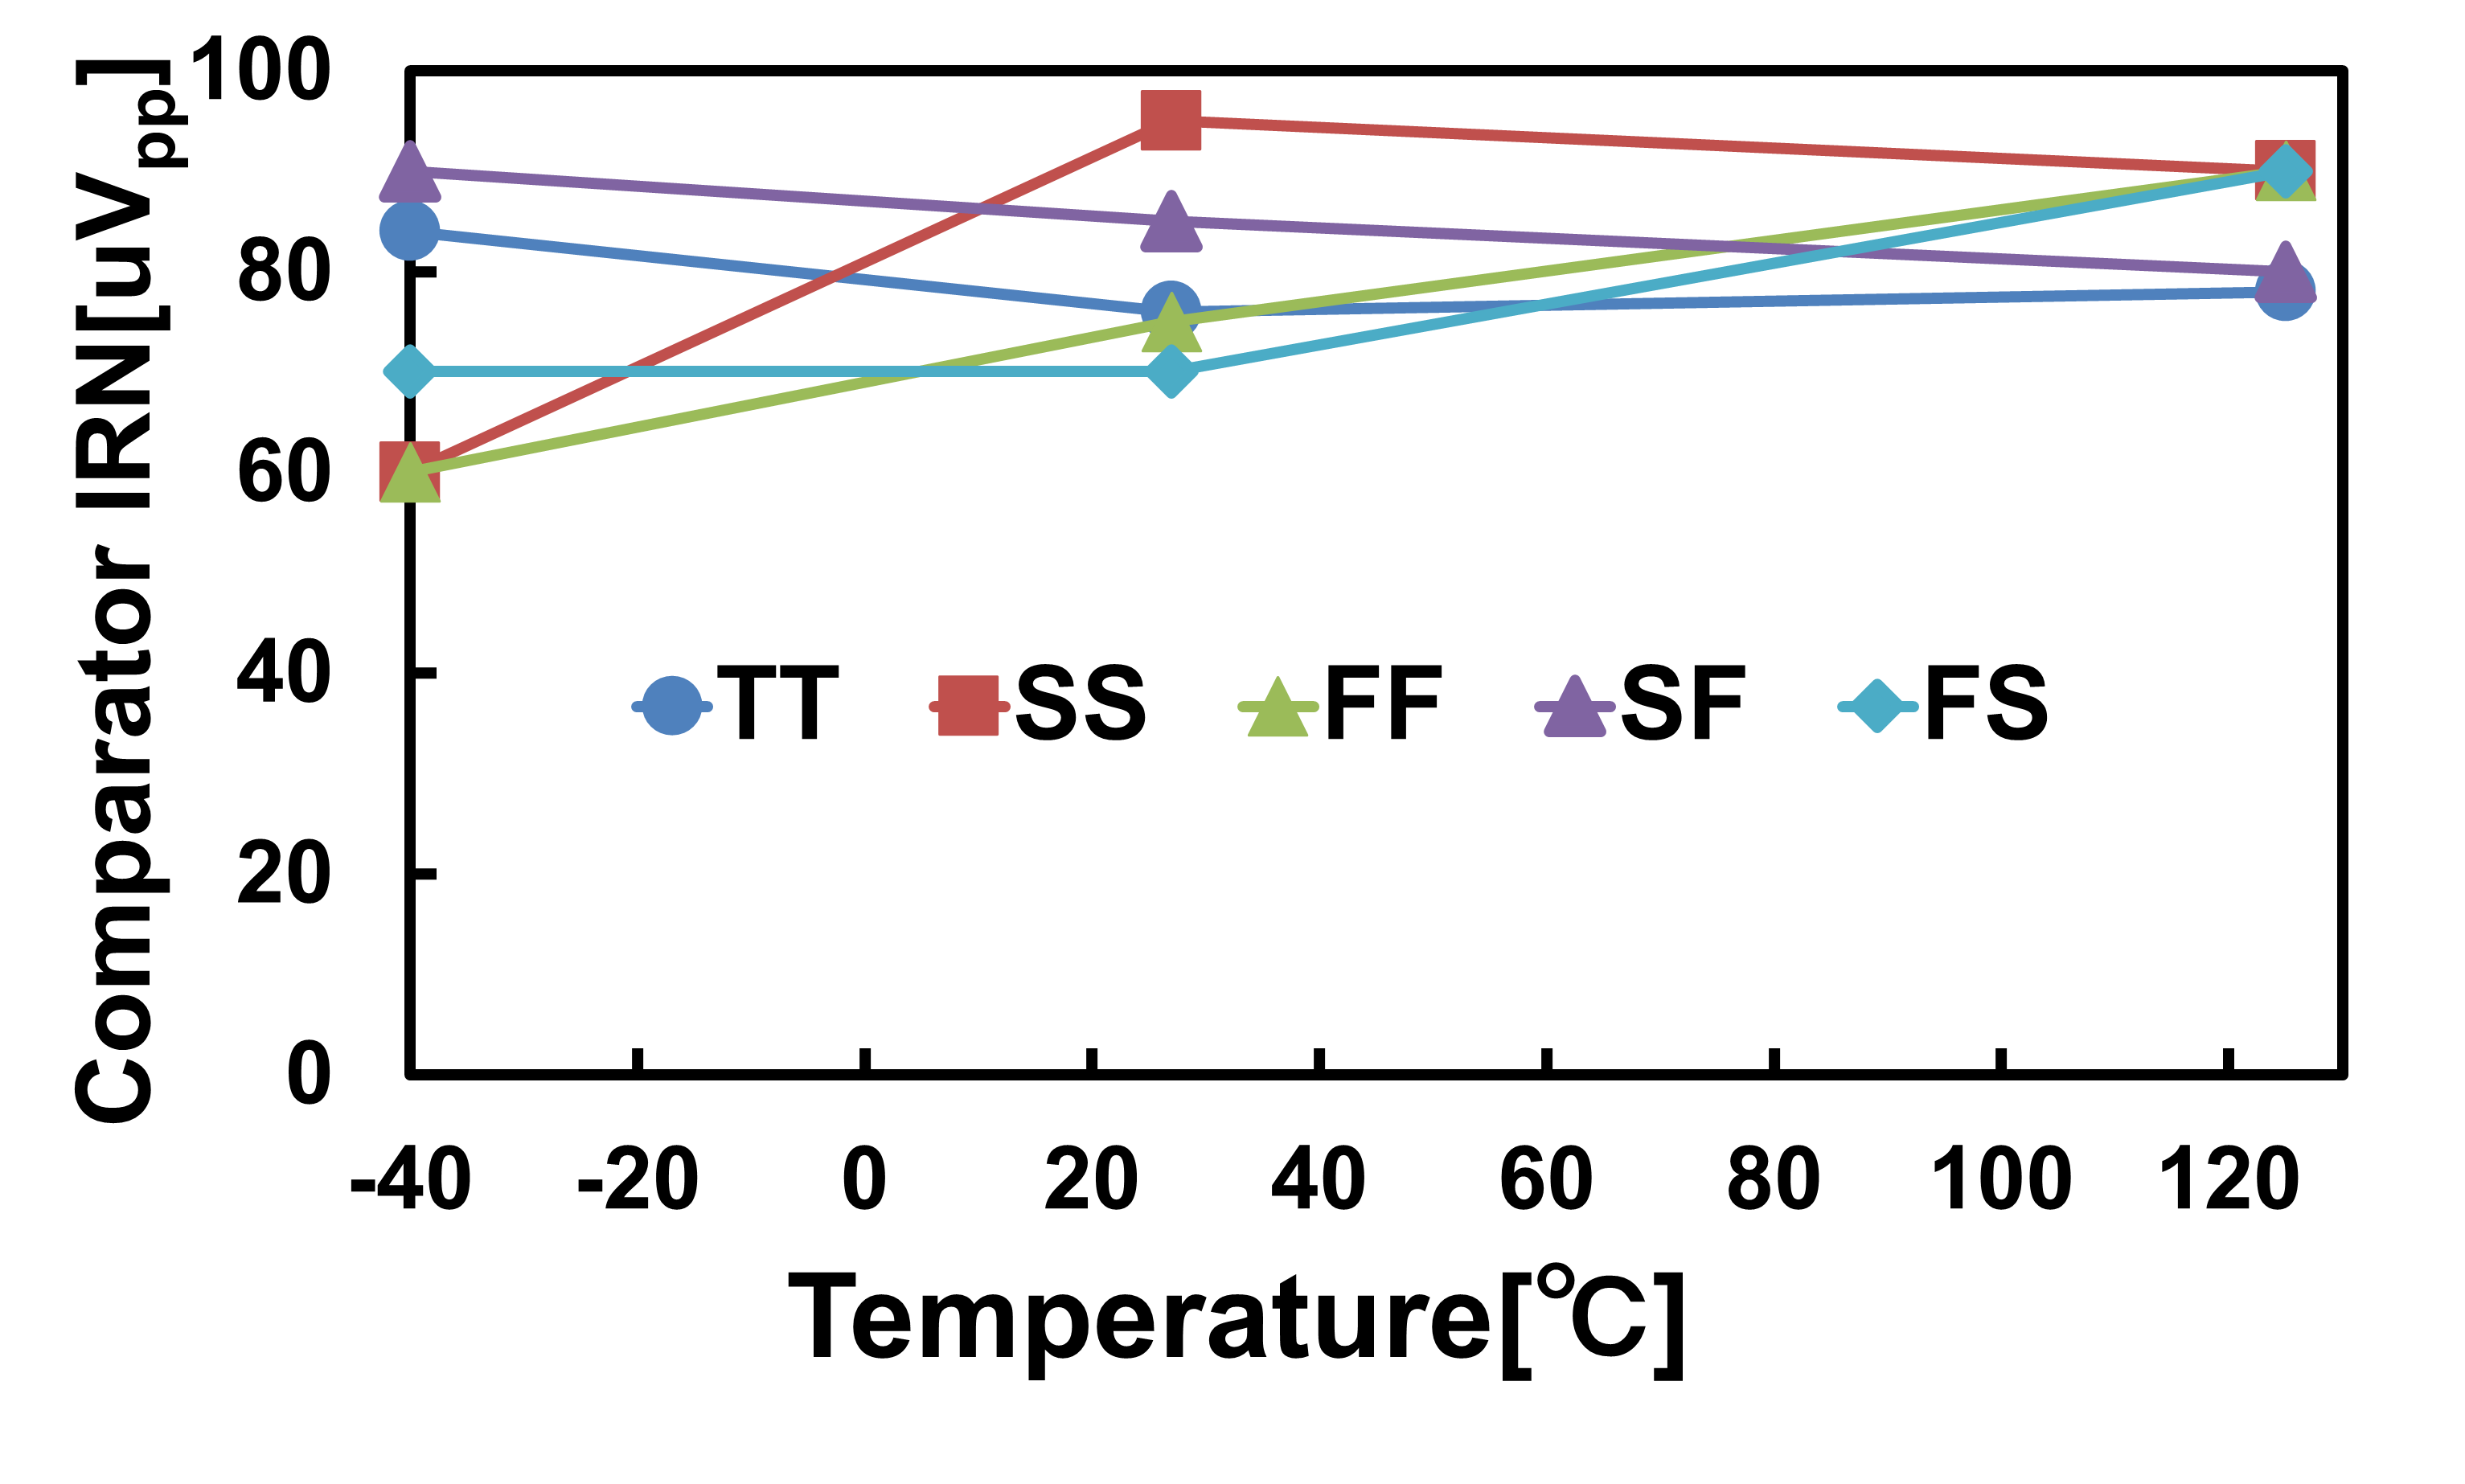
\includegraphics[width=0.5\textwidth]{figs/pvt_vco.png}
  \captionsetup{font=footnotesize}
  \caption{PVTとIRNの関係性}
  \label{pvtvco}
\end{figure}

One of the major issues in high precision comparators is the noise drift due to PVT variations. In general, comparator noise records its worst value at  FF high-temperature corners where current and thermal noise increase. Therefore, it is necessary to suppress the noise under these conditions. On the other hand, the VCO comparator suppresses the noise drift due to PVT variation by exploiting the PVT vs. $g_m$ dependence of the time amplifier.

Eq. (\ref{delaylineIRN}) shows that at FF high-temperature, $IRN_{DL}$ worsens as in normal comparators.
Interestingly, since $G_{TA}$ is inversely proportional to $g_m$, the time amplification gain becomes smaller under FF high-temperature conditions. Thus, the VCO-referred deadzone becomes smaller, which is a shift that improves the IRN of the VCO comparator according to eq(\ref{vcoIRN}). As a result, $IRN_{DL}$ and $G_{TA}$ cancels each other out, and the noise growth at FF conditions can be suppressed. The simulated VCO IRN with PVT variations is shown in Fig.\ref{pvtvco}. Even under the most severe FF high-temperature conditions, the IRN increases only 18\% compared to TT conditions. On the other hand, the noise worsens at SS corners as well, due to the increase in $G_{TA}$. We would like to note that even under this condition, the IRN increase is about 20\% compared to TT conditions.

\subsection{Metastability detection}
Since the comparator accuracy is proportional to the metastable time, high-precision comparators have the risk of conversion errors in asynchronous SAR ADCs. Therefore, metastable detection is necessary.
Conventional comparators often implement metastable detection by directly monitoring the comparison time, but these have a large PVT dependency and require calibration\cite{shikata20120}.

On the other hand, a VCO comparator intrinsically has a metastable detector that does not require PVT calibration; in the case of metastability, the VCO time difference remains within the deadzone and the VCO continues to oscillate. Therefore, metastable detection can be achieved by simply counting the number of oscillations. In our design, the number of VCO oscillations is monitored by a counter circuit, and when the number of oscillations exceeds 10 times, metastability is detected and a random result is stored. By using this intrinsic metastability detection of VCO comparators, we can implement e.g. additional bit judgment \cite{shikata20120,ding20190} and DAC calibration \cite{zhu201914} with less PVT dependency.


\section{Circuit Implementations}
\subsection{13-bit SAR ADC implementation}

\begin{figure*}[ht!]
\centering
 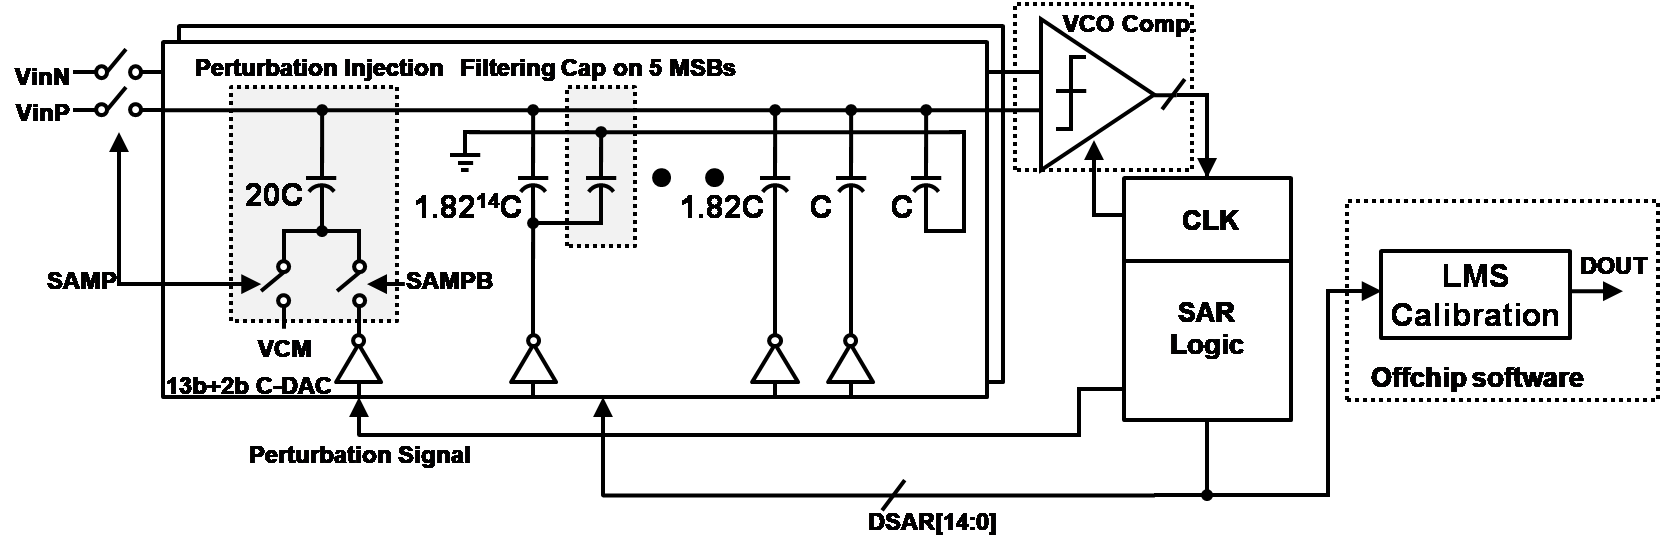
\includegraphics[width=1\textwidth]{figs/fig7.png}
  \captionsetup{font=footnotesize}
  \caption{\textbf{ADC}}
  \label{13bsar}
\end{figure*}

To demonstrate the high-accuracy VCO comparator, we design a proof-of-concept 13-bit low-power SAR ADC.
The entire 13-bit SAR ADC architecture is shown in Fig.\ref{13bsar}. To cut down the C-DAC power, we utilize a sub-binary C-DAC with perturbation logic for LMS calibration as in ref.\cite{liu201012b}. The C-DAC has 2-bit redundancy implemented with a sub-binary radix of 1.82. To suppress the noise of C-DAC buffers, filtering capacitors\cite{miki20154} are provided until the 5th MSB bit. Unit capacitor (C) of 0.5fF was chosen to meet the kT/C noise requirements.

To cancel the capacitor mismatch effect, perturbation-based digital calibration\cite{liu201012b} is employed. When the calibration is active, two conversions are resolved for the same sample. The conversions are perturbed with an offset of $\pm \delta$ is injected before the SA cycle starts. The perturbation injecting capacitor is 20C as shown in Fig.\ref{13bsar}. After the first conversion ends, the perturbation signal is inverted so that it will inject with different polarity. In this work, the LMS calibration engine was implemented fully off-chip.

\subsection{VCO-based comparator with multiple noise modes}
\begin{figure}[ht!]
\centering
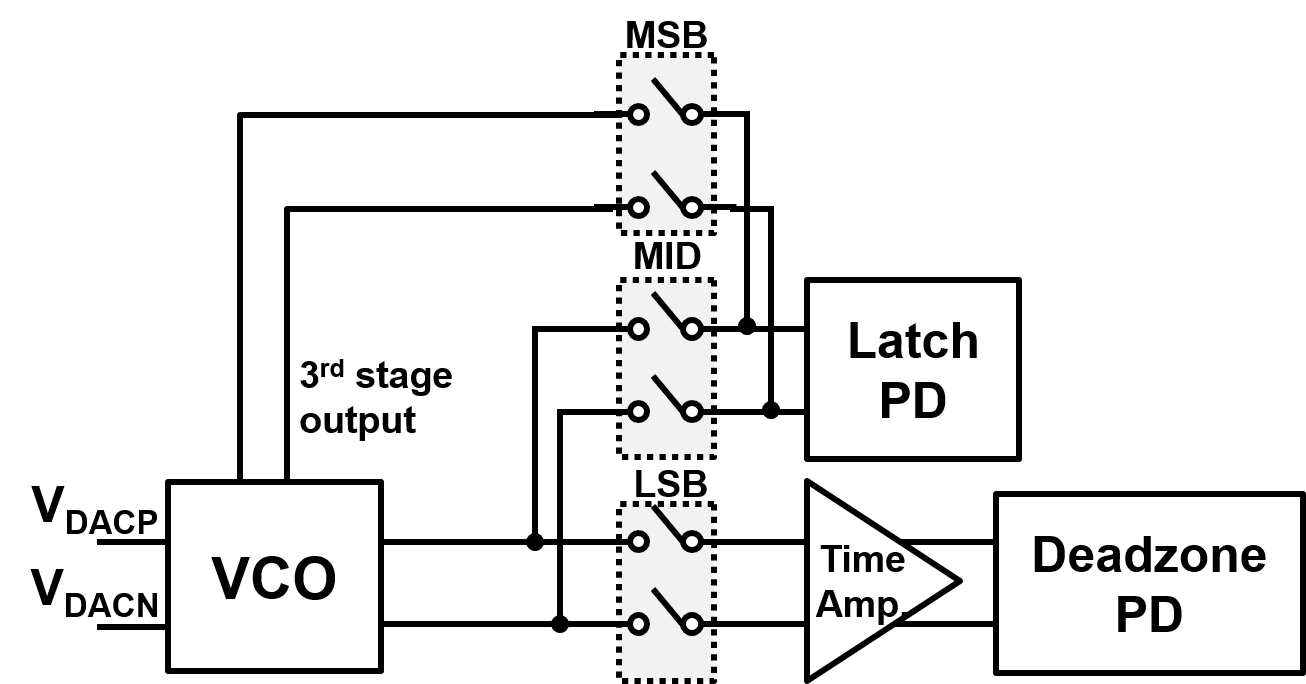
\includegraphics[width=0.5\textwidth]{figs/vco-entire.png}
\caption{\textbf{ADC}}
\label{fullvco}
\end{figure}

High-precision SAR ADCs are often designed with redundancy to mitigate the effects of DAC and reference settling. Since the comparator noise requirements differ according to the SA cycles, it is useful if the comparator noise mode can be digitally configured.
Our 13-bit SAR ADC holds 2-bit redundancy: since redundancy is assigned to each bit, even if a judgment error occurs in the upper bits, errors can be corrected with fine bit decisions in the LSB comparisons\cite{kapusta201314b}. For example, the upper 5 bits can tolerate a decision error equivalent to 200 LSBs. It would be a waste of energy to use a VCO-based comparator with sub-LSB accuracy in the MSBs.

As in Fig.\ref{fullvco}, we propose a VCO comparator mechanism with digitally configurable noise performance. 
The main idea is to use a delay line-based comparator with a feed-forward latch to minimize power consumption during MSB comparisons, where accuracy is not required. During LSB comparisons, we switch to a VCO-based comparator with deadzone PDs.
A simple switching circuit allows the VCO comparator to have three noise modes in a small area. The specific implementation is as follows:
\begin{itemize}
\item \textbf{MSB mode} (first 5 SA cycles): Operates as a simple 3-stage delay line. MSB mode: Operates as a simple 3-stage delay line, since it can tolerate large judgment errors. IRN:2mVpp.
\item \textbf{MID mode} (middle 5 SA cycles): Operates as an 11-stage delay line. IRN:180uVpp.
\item \textbf{LSB mode} (last 5 SA cycles): 11-stage VCO operation as described in Chapter 3. IRN:80uVpp.
\end{itemize}
In the MSB and MID modes, latch-based PD is used to force decisions with positive feedback. Such PDs are noisier, but do not have deadzones, and are power-efficient.

\subsection{VCO and Time Amp. designs}
\begin{figure}[ht!]
\centering
 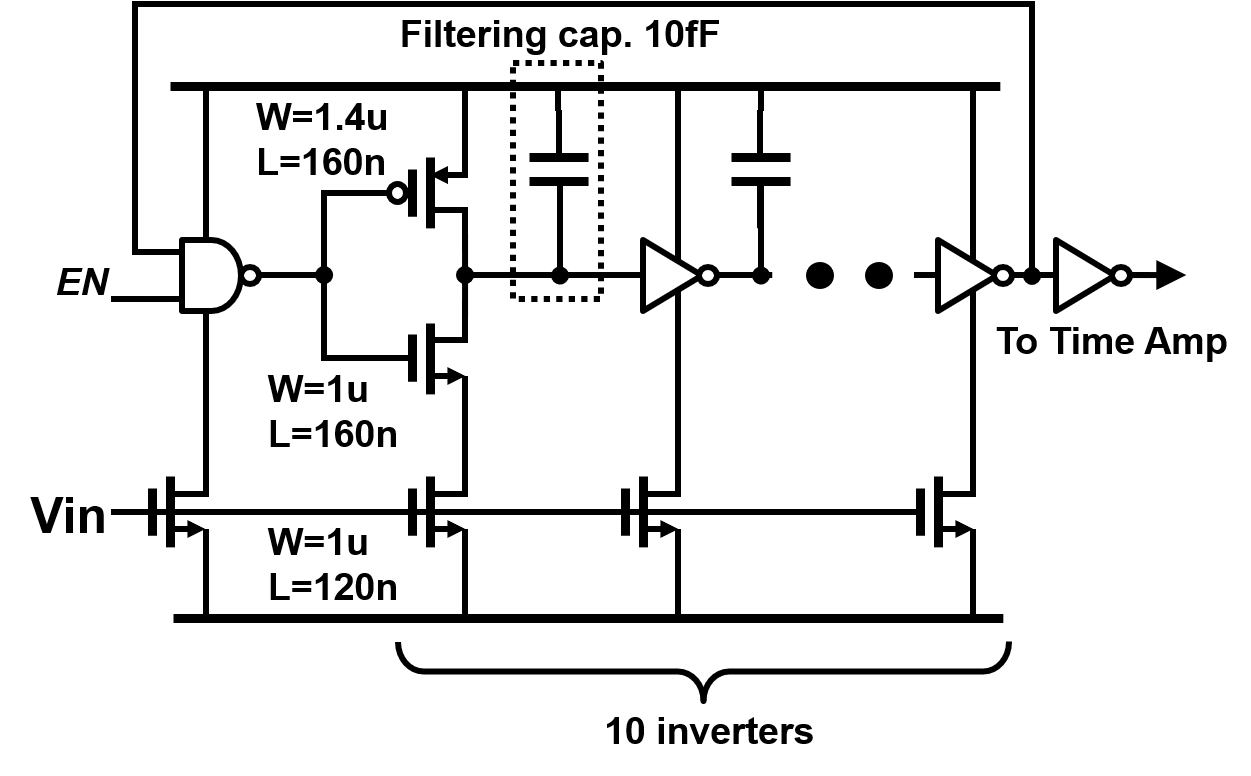
\includegraphics[width=0.5\textwidth]{figs/vco_cell.png}
  \captionsetup{font=footnotesize}
  \caption{\textbf{ADC}}
  \label{cell}
\end{figure}

\begin{figure}[ht!]
\centering
 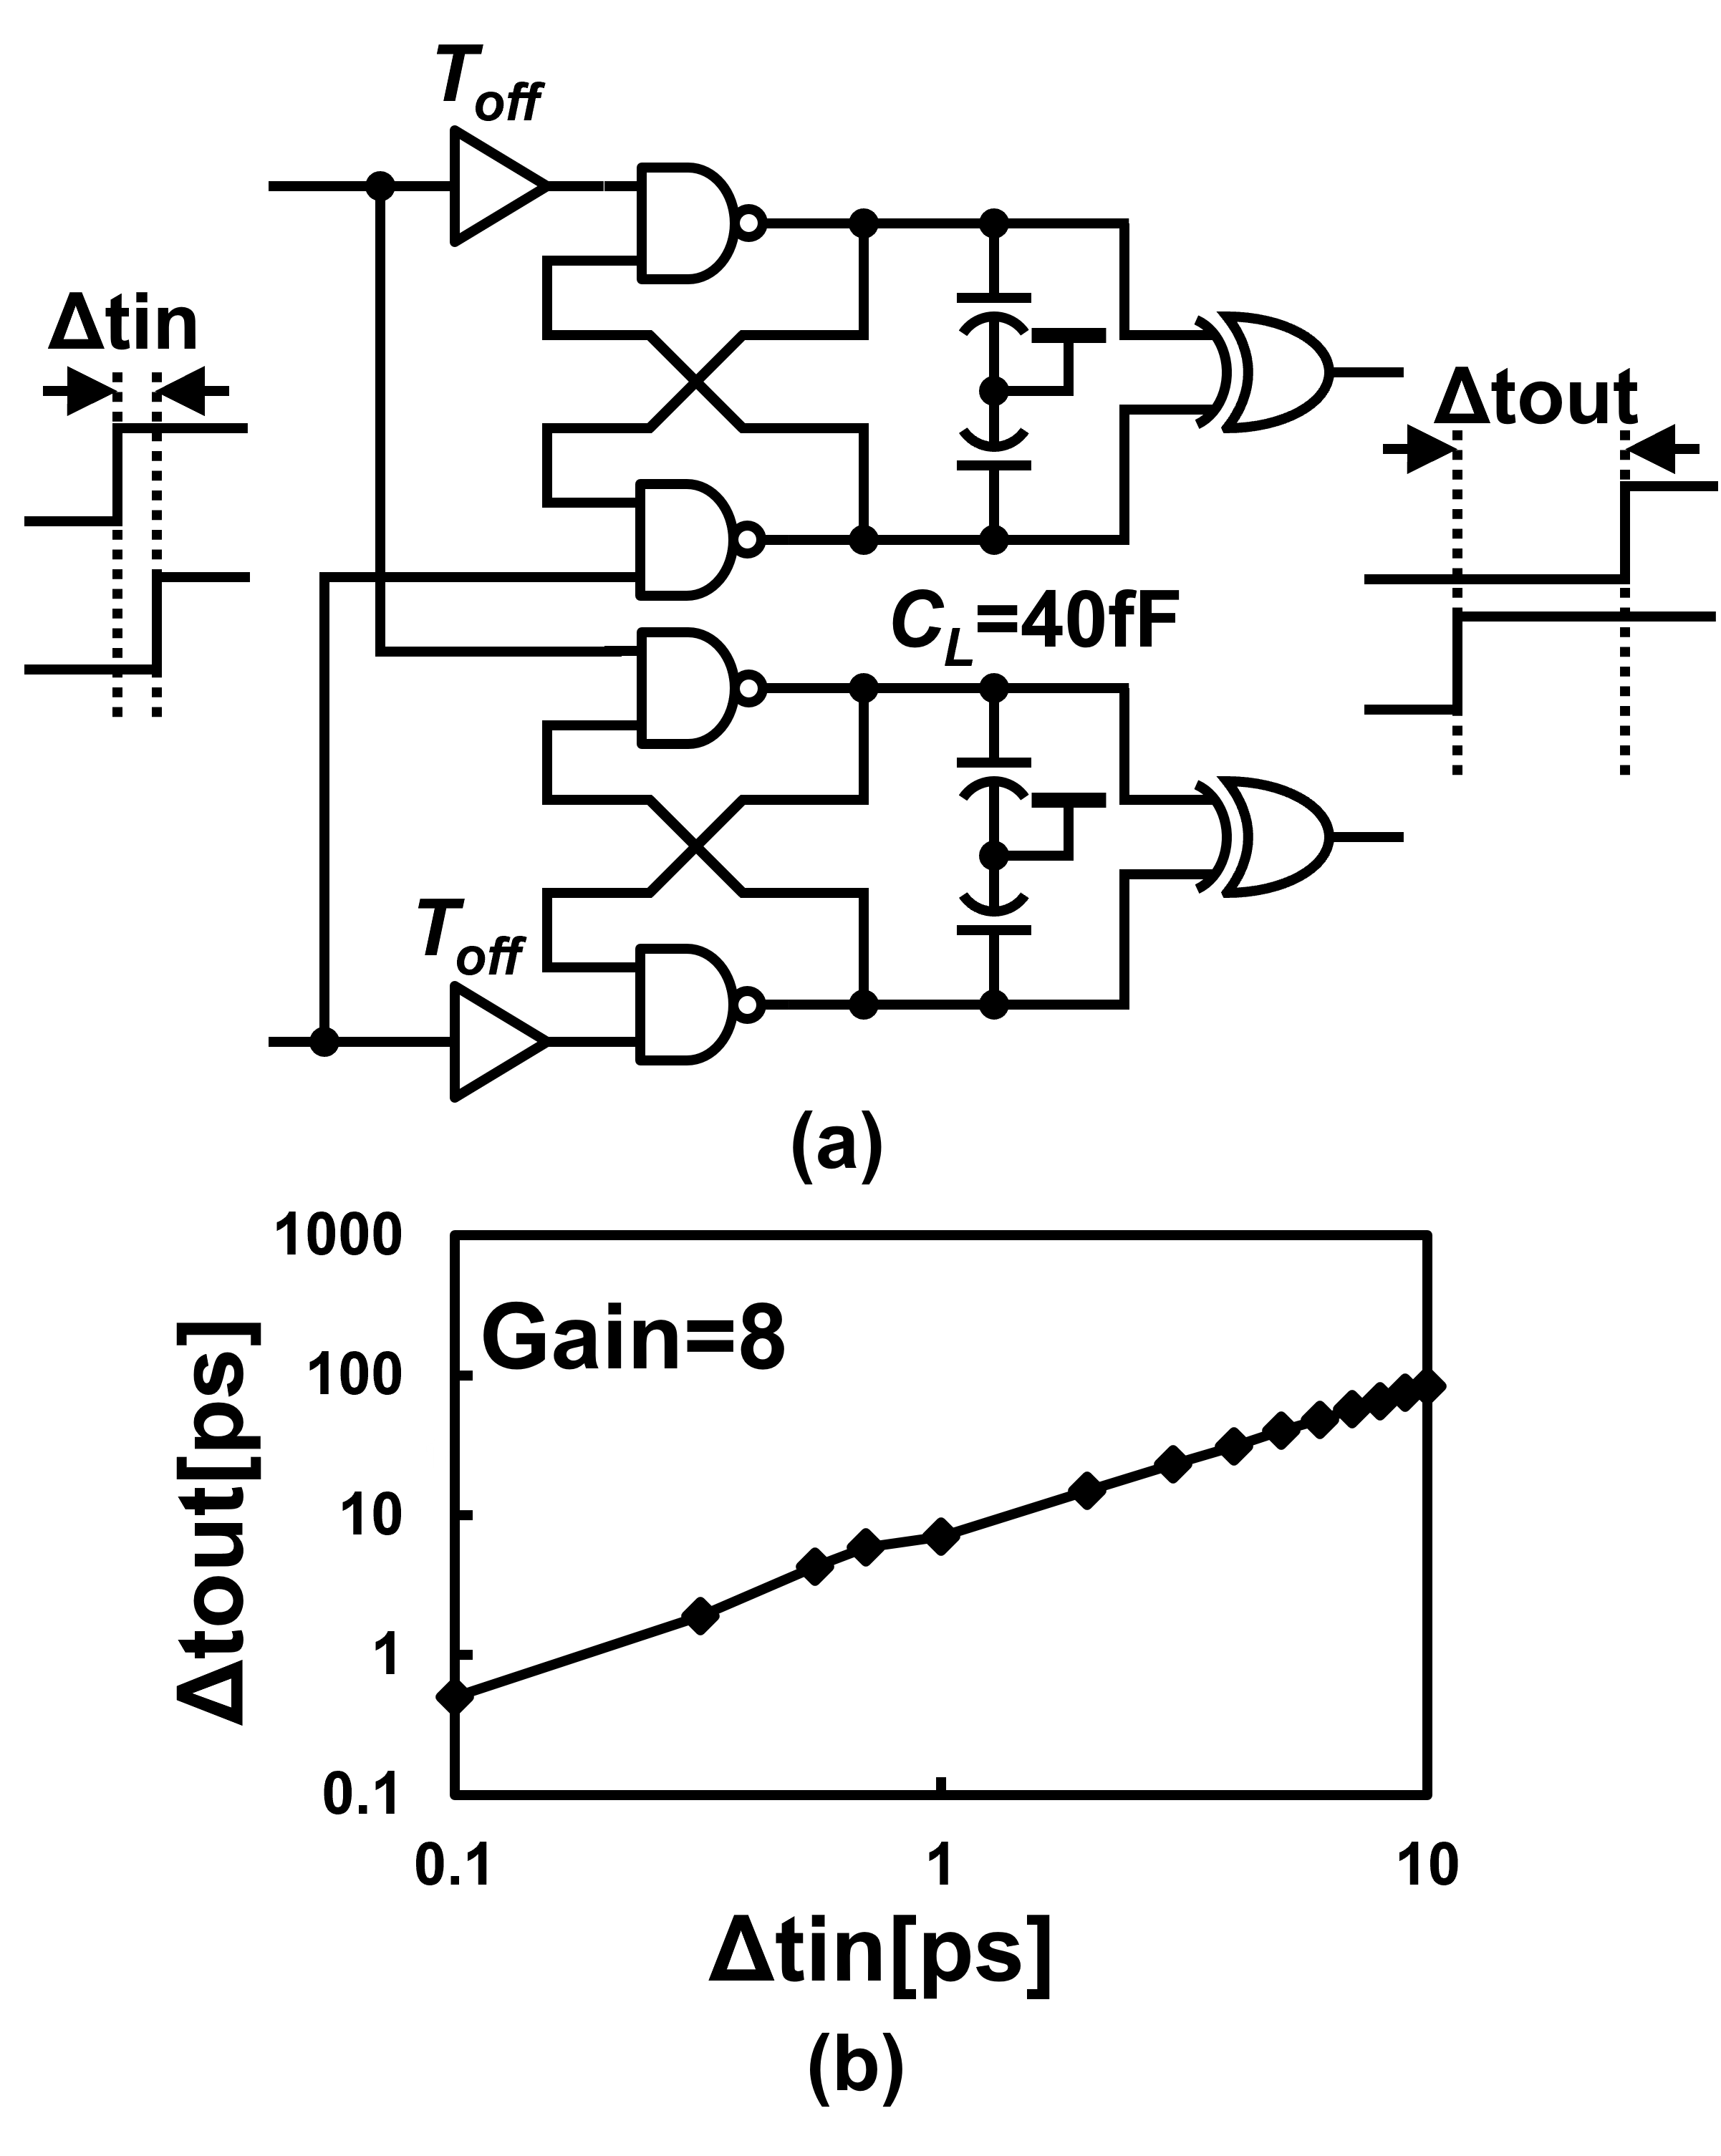
\includegraphics[width=0.5\textwidth]{figs/ta_chara.png}
  \captionsetup{font=footnotesize}
  \caption{\textbf{ADC}}
  \label{timeamp}
\end{figure}

Finally, we describe the design of the VCO cell and time amplifier. As shown in Fig.\ref{cell}, the VCO cell achieves voltage-time conversion by binding the NMOS side of the inverter in a current-starving fashion. As in ref.\cite{timecomp}, the PMOS side can also be current-starved to increase the VCO voltage-time conversion gain, which improves the noise performance. However, when the PMOS is also tied, the VCO oscillation frequency dropped significantly and was not suitable for our target of 1MS/s SAR ADC operation. The VCO in this design is designed to oscillate at 600MHz when a common-mode voltage (500mV) is given, which is a sufficient speed for 1MS/s SAR ADCs. While the tail NMOS $g_m$ should be maximized to suppress noise, the gate leakage currents contributed to the accuracy degradation in our design. Thus, the L sizing was increased to mitigate this effect. 

Our time amplifier is designed based on ref.\cite{lee20089}, and the schematics and simulated amplification characteristics are shown in Fig.\ref{timeamp}. Although the nonlinearity is noticeable, it does not affect the accuracy of the comparator as long as the monotonicity is maintained.
Also, $G_{TA}$ is given by
\begin{eqnarray}
    \centering
    G_{TA} = \frac{2C_L}{g_mT_{off}}
    \label{gta}
\end{eqnarray}
As mentioned in the previous section, under FF high-temperature conditions $G_{TA}$ drops, since the gain is inversely proportional to $g_m$.
In this design, the gain at TT condition is designed to be 8 by tuning $T_{off}$ and the load capacitance. Moreover, while not implemented in this design, $G_{TA}$ can be easily configured by digitally switching $C_L$. By such mechanisms, we can digitally control the noise performance of the VCO comparator and such configuration can become useful when designing ADCs for multiple resolution modes\cite{harpe201310b}.

% ここまで書いた
\section{Experiment Results}
\begin{figure}[ht!]
\centering
 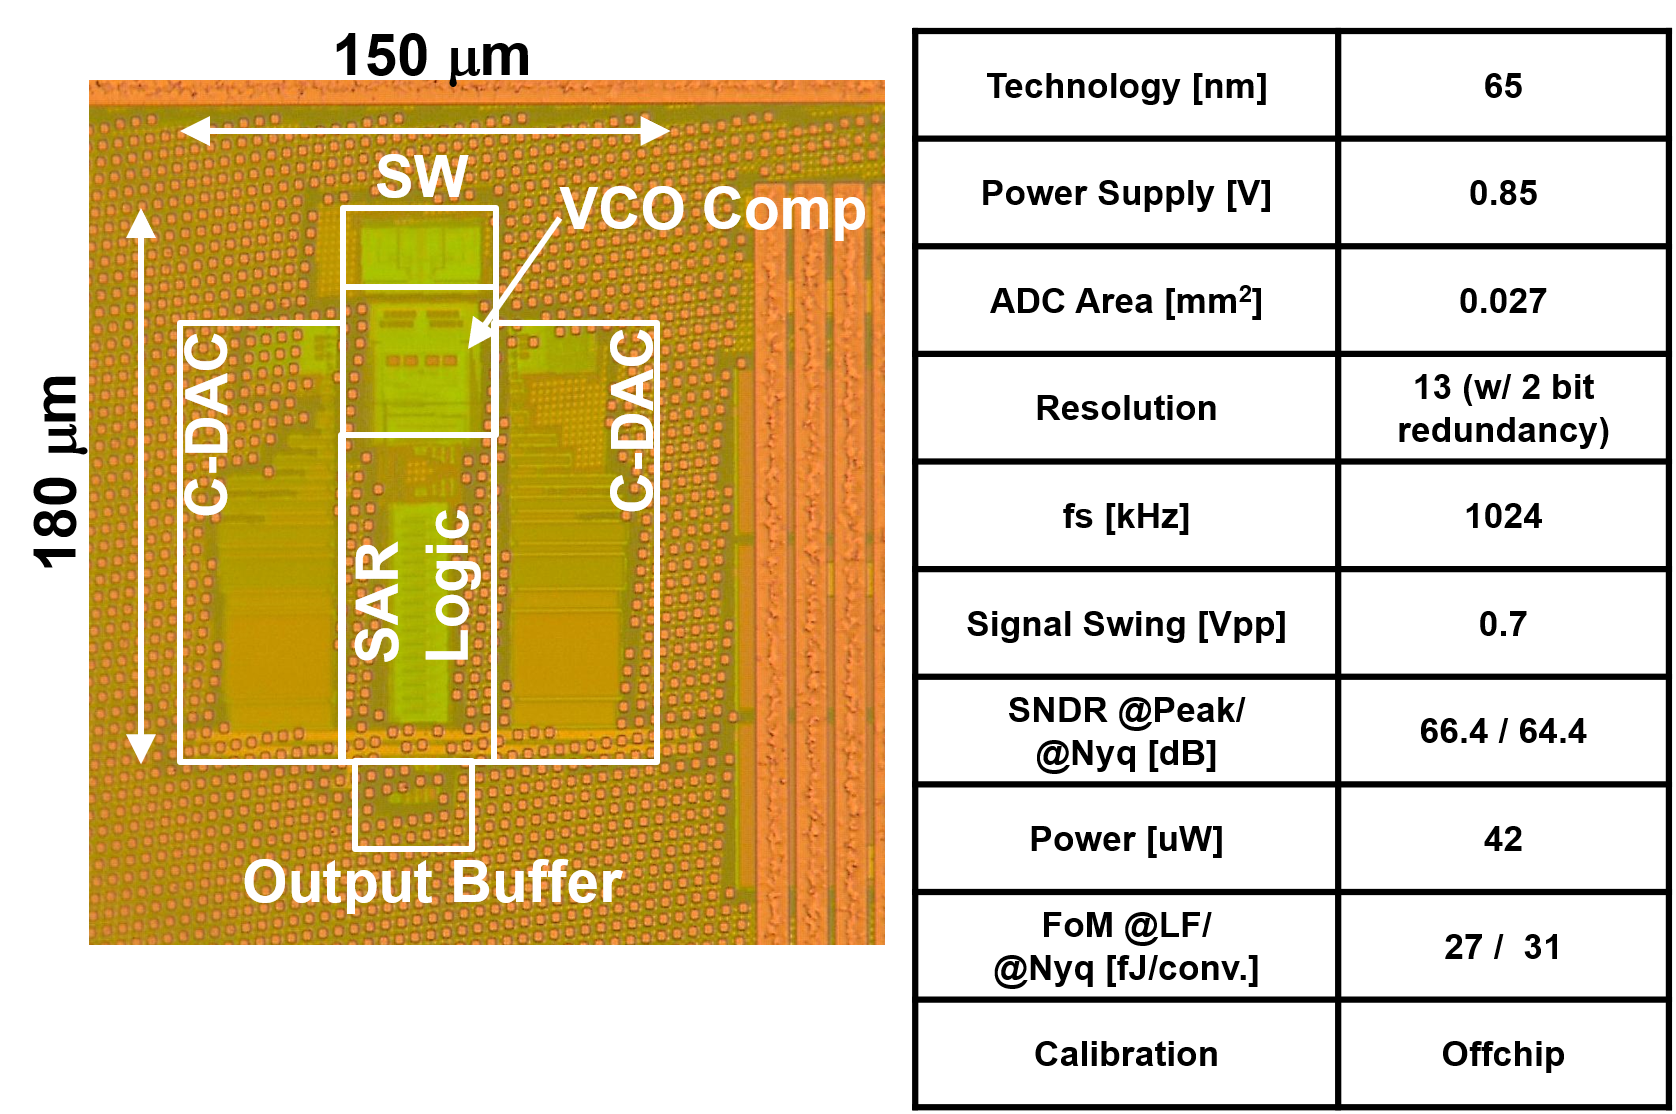
\includegraphics[width=0.5\textwidth]{figs/chipphoto.png}
  \captionsetup{font=footnotesize}
  \caption{Chip micrograph and performance summary of the ADC.}
  \label{chipphoto}
\end{figure}

\begin{figure}[ht!]
\centering
 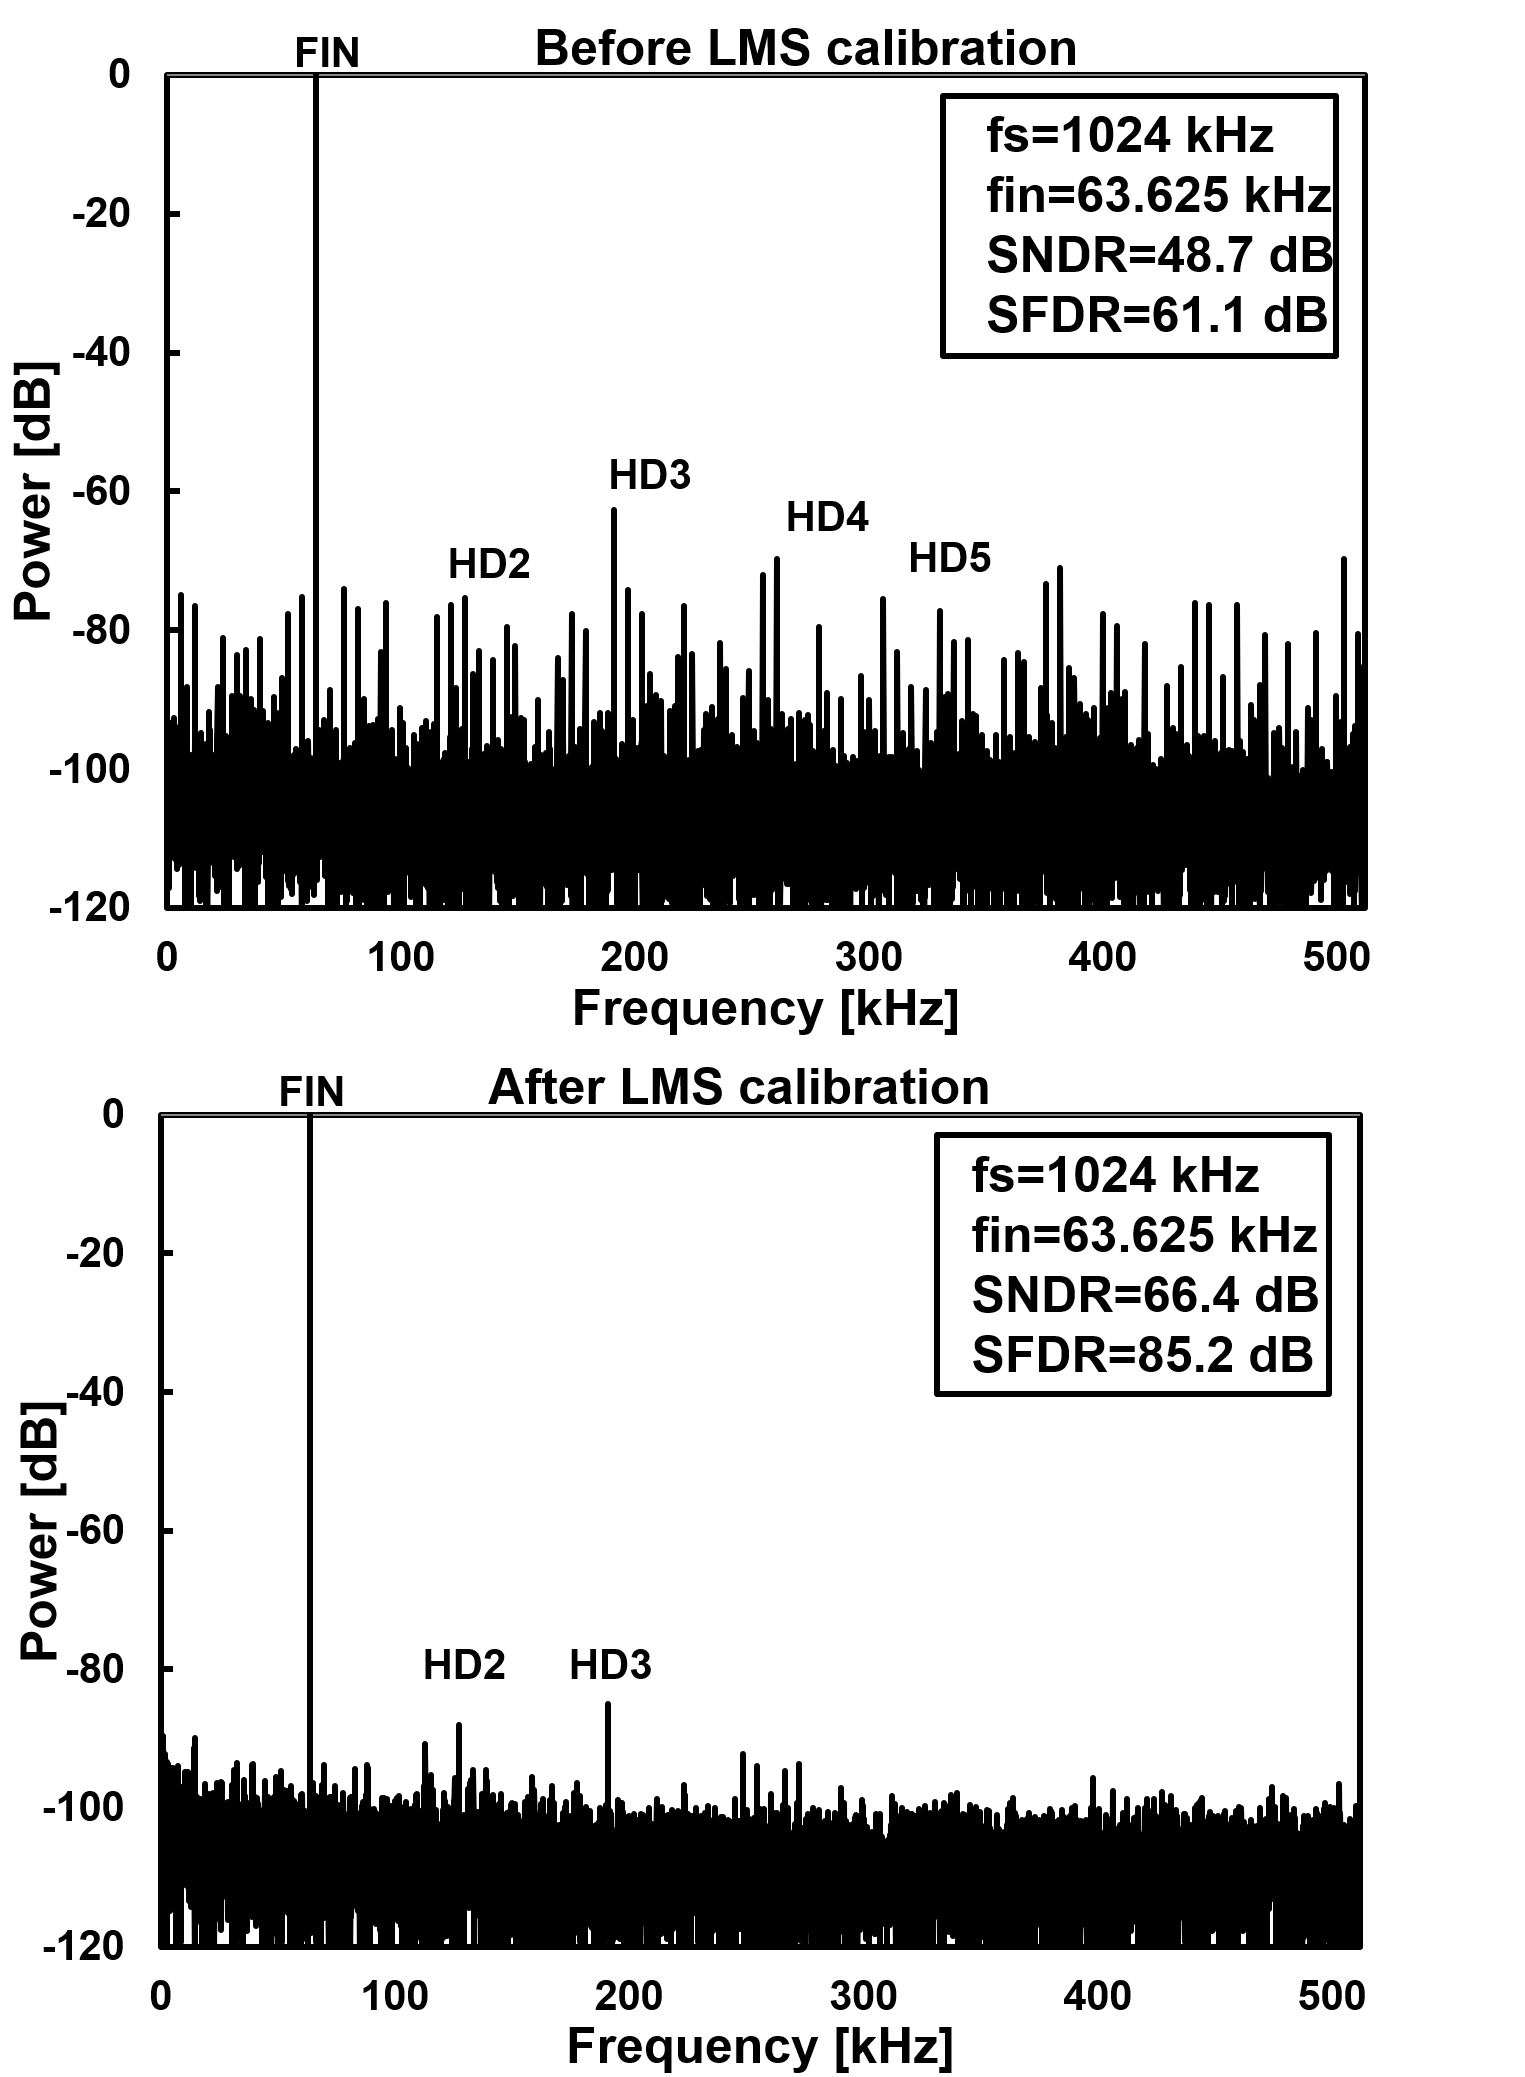
\includegraphics[width=0.5\textwidth]{figs/fft.png}
  \captionsetup{font=footnotesize}
  \caption{16384 FFT results before and after calibration.}
  \label{aftercal}
\end{figure}

\begin{figure}[ht!]
\centering
 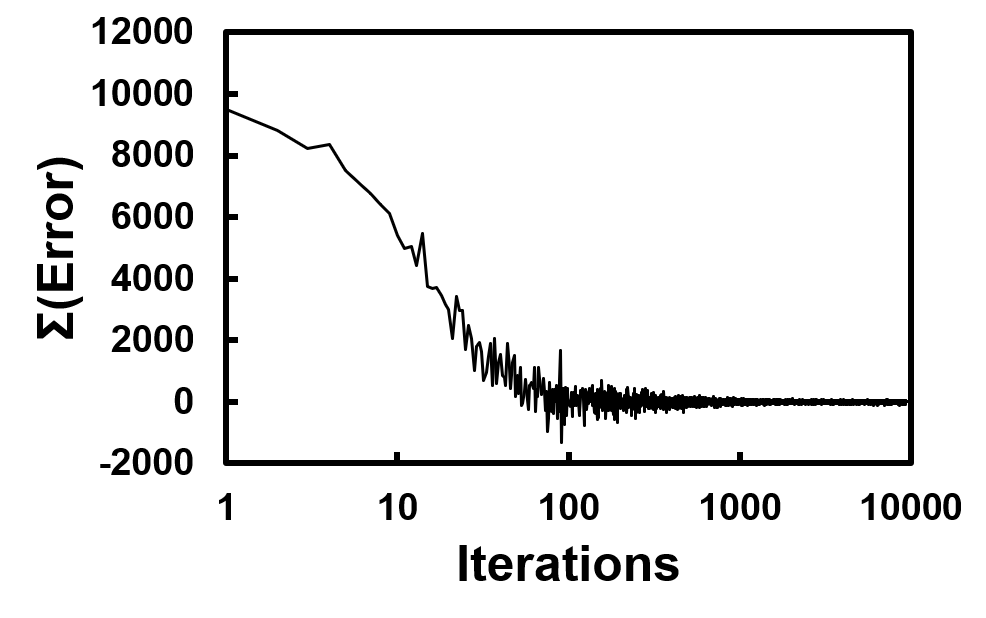
\includegraphics[width=0.5\textwidth]{figs/lms.png}
  \captionsetup{font=footnotesize}
  \caption{LMS calibration error convergence.}
  \label{lms}
\end{figure}

\begin{figure}[ht!]
\centering
 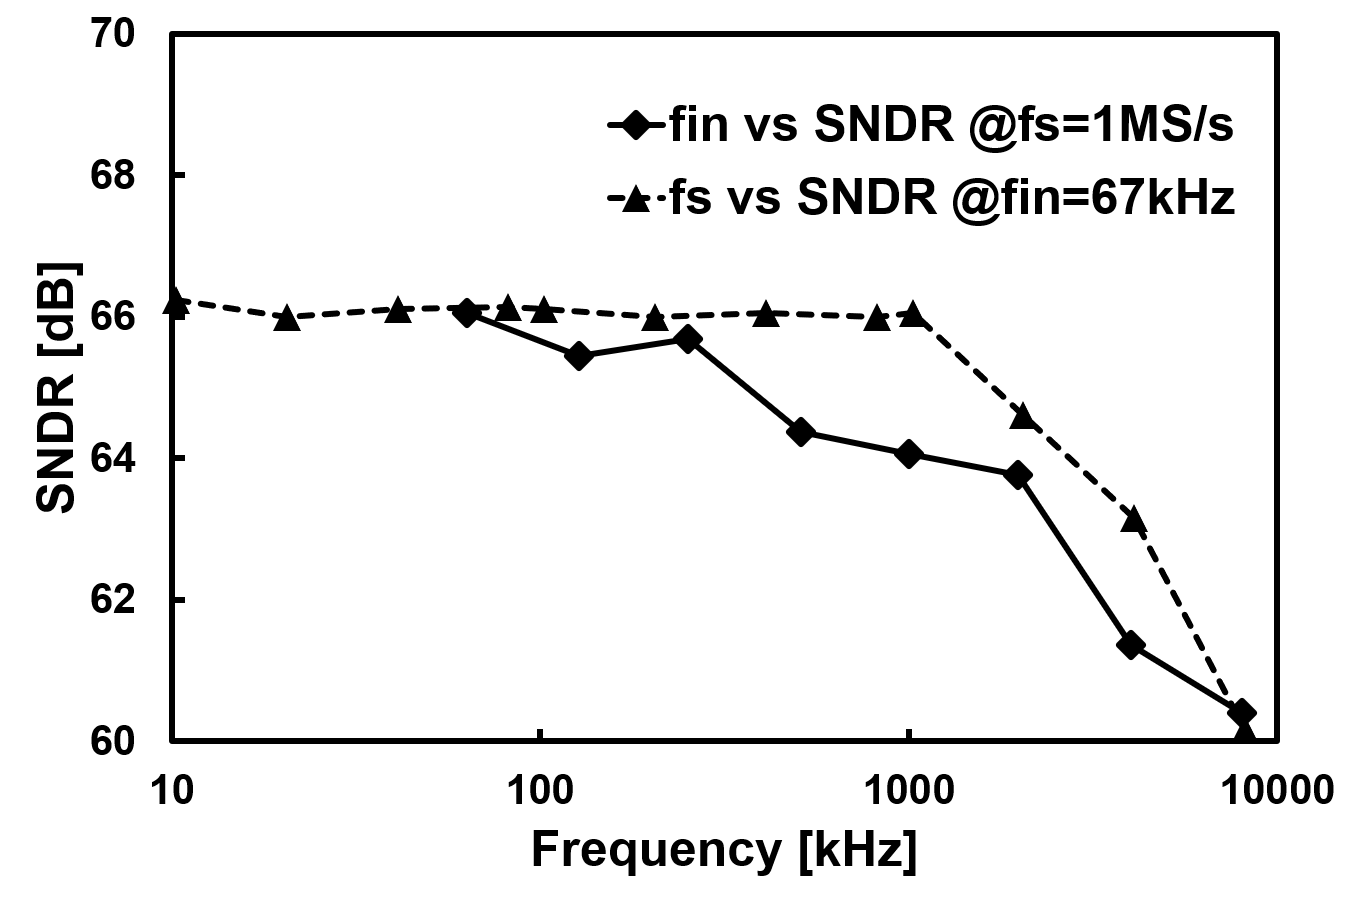
\includegraphics[width=0.5\textwidth]{figs/freq-sndr.png}
  \captionsetup{font=footnotesize}
  \caption{Measured fin and fs versus SNDR characteristics, respectively.}
  \label{freqvssndr}
\end{figure}

\begin{table*}[ht!]
\centering
 \caption{Performance comparison between low-power SAR ADCs.}
 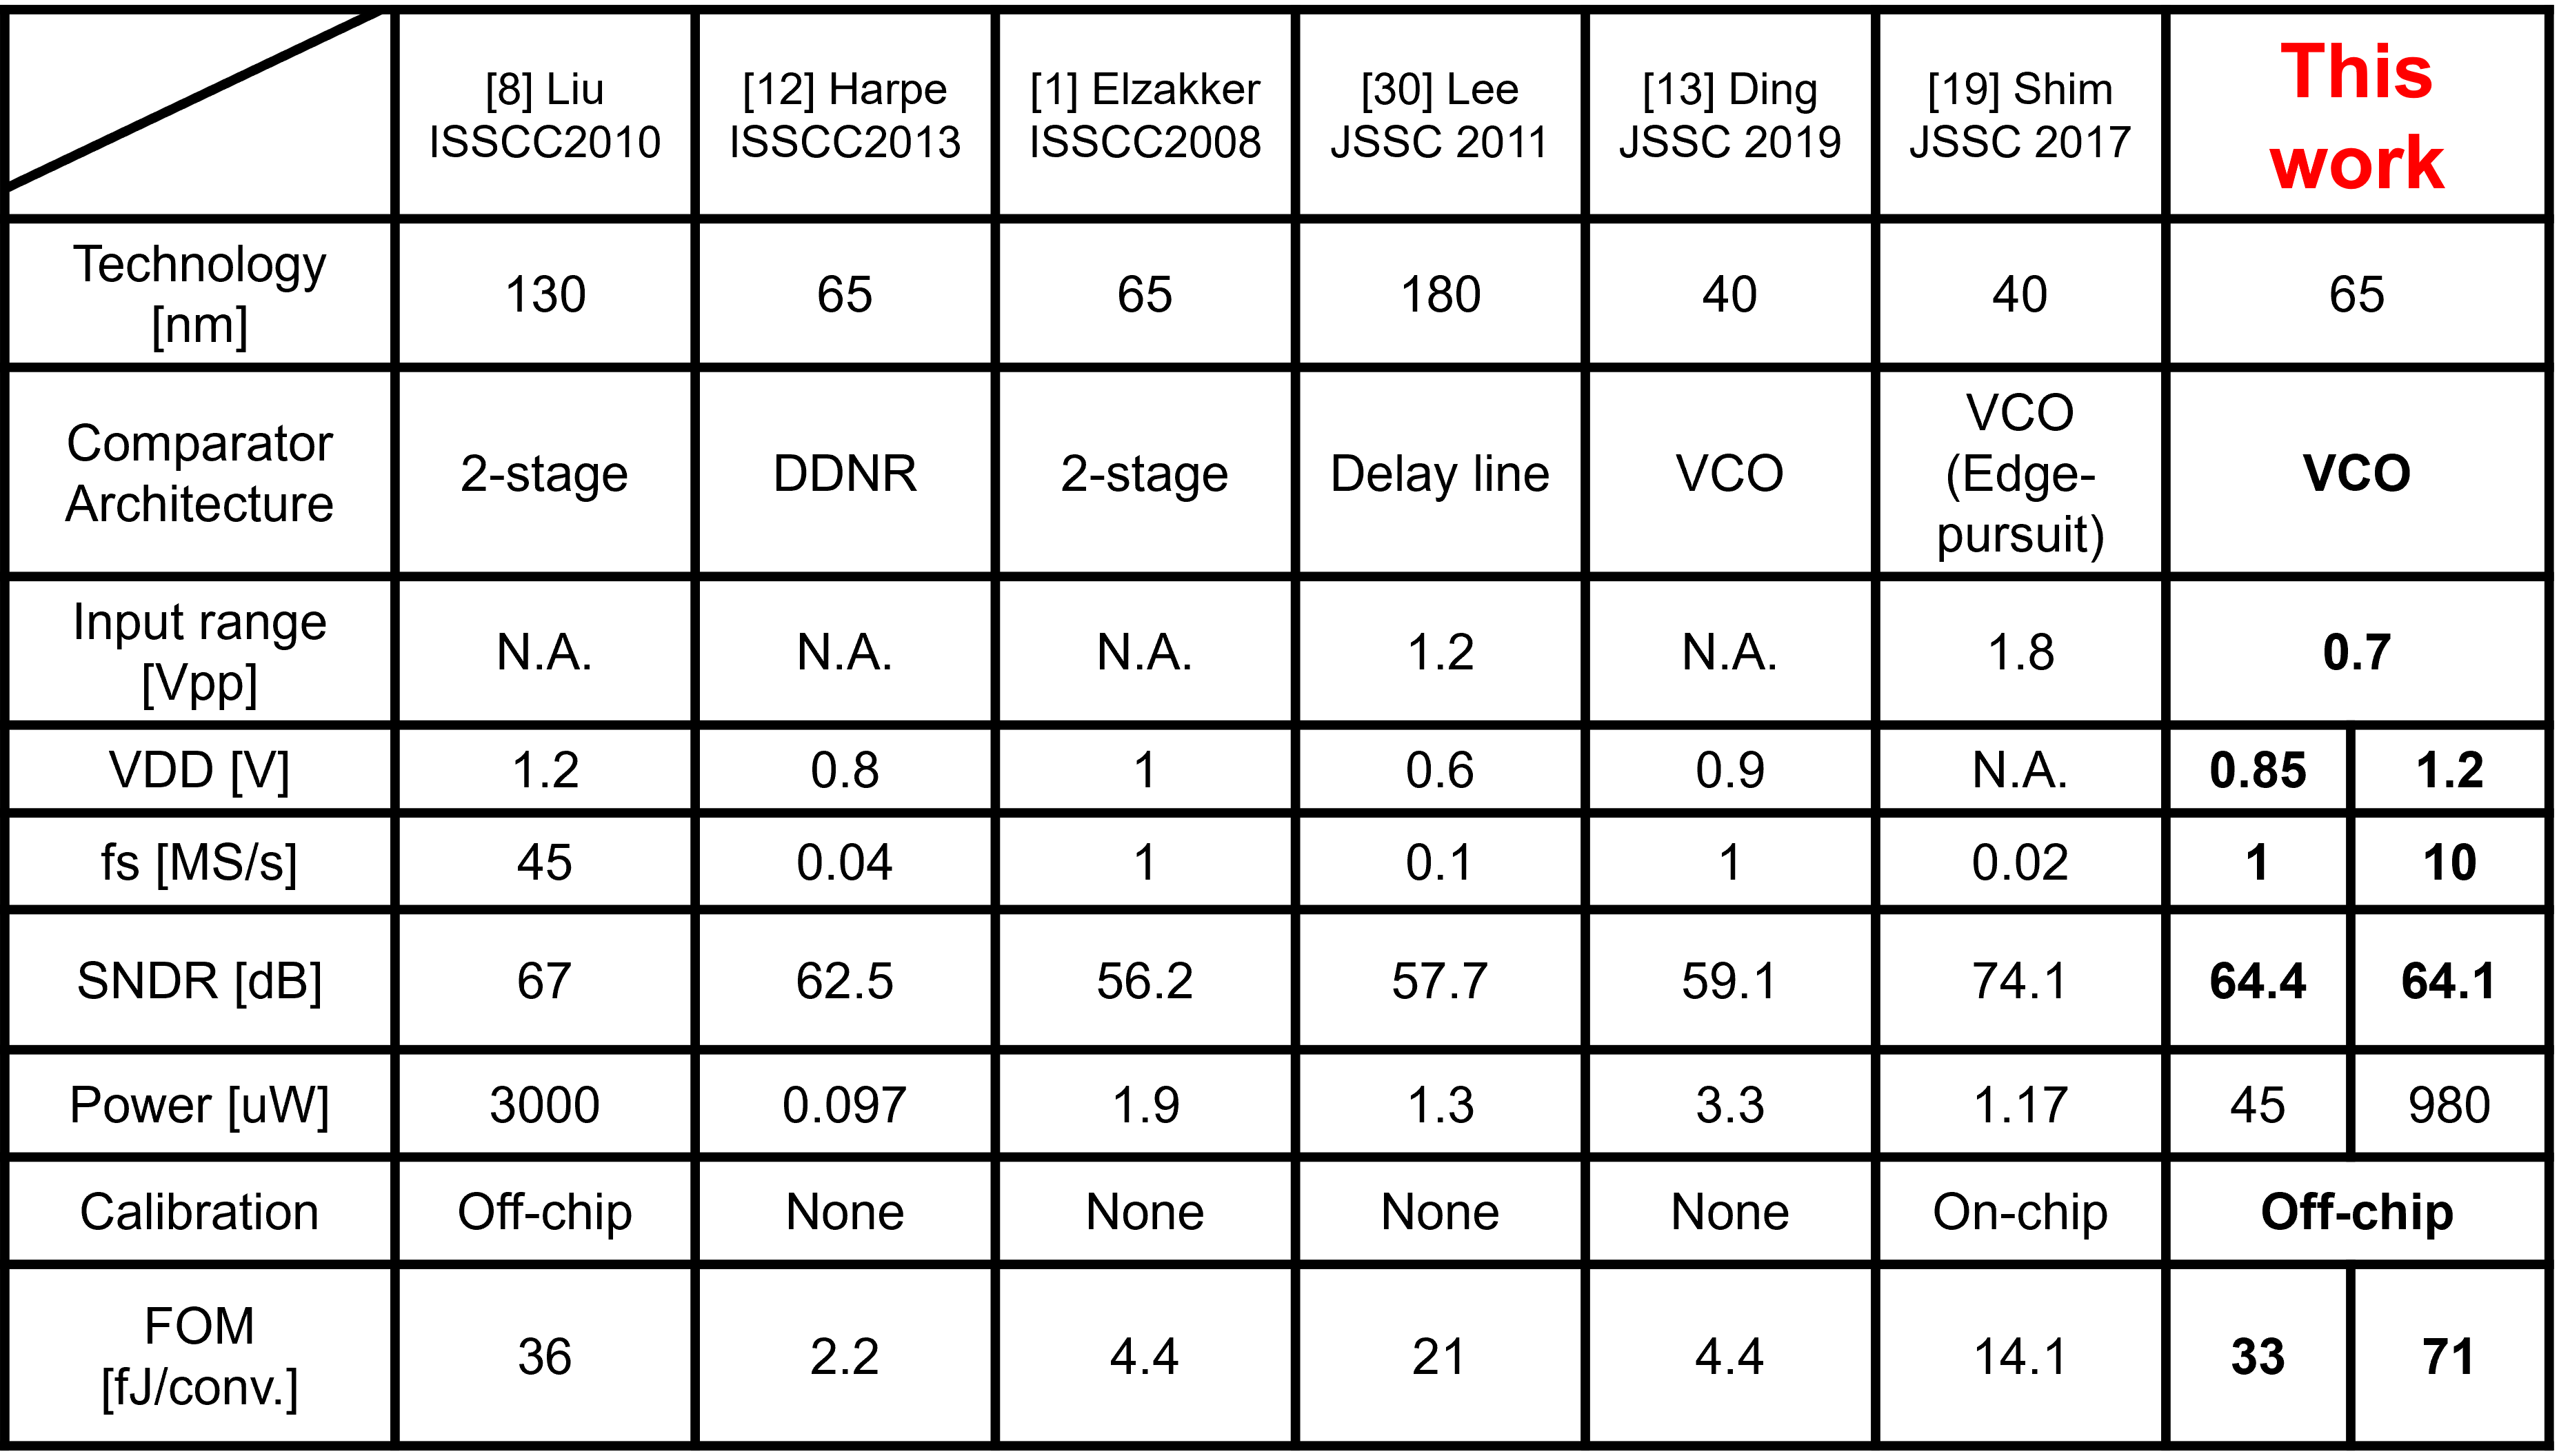
\includegraphics[width=0.9\textwidth]{figs/table.png}
  \captionsetup{font=footnotesize}
  \label{performancecomp}
\end{table*}

The SAR ADC was fabricated in 65-nm CMOS and Fig.8 shows the chip micrograph and a performance summary. 
Fig.\ref{aftercal} shows the result of 16384-FFT before and after LMS calibration. The two FFT results were lead using the same raw data, but different bit weighting was used: the prior uses the weighting as in the schematic and the latter uses weighting derived via LMS calibration. Therefore, the noise situation is the same. Even though we do not add any tuning to the VCO-based comparator in this design, fine noise performance was achieved. 

Fig.\ref{lms} shows the calibration iteration versus the error convergence. With sufficient hyper-parameters, the LMS engine requires about 5000 iterations for convergence. After that, the perturbation injection can be stopped to save power. 
We plot fs and fin versus SNDR respectively in Fig.\ref{freqvssndr}. Since the VCO-based comparator is mostly digital, low voltage operation was easily accomplished. All of the measurements have been carried out with a single supply voltage of 0.85V. At 1.2V supply, the ADC achieves similar SNDR performance and extends fs to 10MS/s, but with a worsened power efficiency. In addition, we must be careful of the signal common-mode voltage ($V_{CM}$) since this directly impacts the inverter’s $I_{DS}$ in eq.(\ref{delaylineIRN}). When the $V_{CM}$ was increased beyond 0.5V, degradation in SNDR was observed.

Finally, we conduct a performance comparison with low-power SAR ADCs in Table \ref{performancecomp}. Our SAR ADC is the first to achieve fully adaptive noise scaling for high-resolution comparators, which opens a new field of research upon further power reduction of the comparator power consumption. 
One of the reasons why the power consumption was inferior to other state-of-the-art ADCs was due to limitations in the measurement environment. Due to the poor IP3 performance of the signal generator, the signal input swing was limited to $0.7V_{pp}$, which occupies only half of the SAR ADC input range. Even with LMS calibration, the SNDR was limited to 66.4 dB but achieving full-scale input should further extend the SNDR around 3-4dB. We would like to note that the power consumption shown in Fig.\ref{chipphoto} is measured when the perturbation injection is turned off. If the LMS calibration engine was to be implemented on-chip and run background, we expect that the total power consumption will increase 3x. 

\section{Conclusions}
To realize a fully adaptive noise scaling comparator, a VCO-based comparator with an eye-opening operation was introduced.  Even though the proposed VCO-based comparator was designed for a 13b ADC, this comparator can be used for further resolutions by carefully designing the jitter performance and the effective deadzone size. Moreover, since this comparator is mainly based on inverters and other simple logic cells, the comparator receives full benefits from process scaling. %Furthermore, the comparator characteristics can be analyzed with well-known knowledge of ring-oscillators. 

\bibliographystyle{IEEEbib}
\bibliography{main}


\begin{IEEEbiography}
[{
\includegraphics[width=1in,height=1.25in,clip,keepaspectratio]{bio/1.jpg}}]{Kentaro Yoshioka}
received his BS, MS, Ph.D degrees from Keio University, Japan. Currently, he is an Assistant Professor at Keio University. He worked with Toshiba during 2014-2021, developing circuitry for WiFi and LiDAR SoCs. During 2017-2018, he had been a visiting scholar at Stanford University, exploring efficient machine learning hardware and algorithms. 

Currently, Dr. Yoshioka serves as a technical program member of Symp. VLSI circuits conference. He was the recipient of ASP-DAC 2013 Special Feature Award, the A-SSCC 2012 Best Design Award, and 1st place winner of Kaggle 2020 Prostate Cancer Grade Assessment (PANDA) Challenge.
\end{IEEEbiography}

\end{document}
